\chapter{NEOS}
\red{need to rename the names everywhere for bce and neos}
This chapter compares the \ac{neos} approach to established methods by evaluating upper cross-section limits on the boosted \ac{vbf} $HH\rightarrow4b$ analysis. This section is not intended to find the most stringent cross-section limits but rather to provide a fair comparison and present the potential \ac{neos} holds compared to more conservative methods.

also what to see what happens when everything is turned on simulatenosuly as doing autoanalysis.

alles ist für k2v0 optimiert, say in traingin?

Specifically, \ac{neos} is compared against cross-section upper limits retrieved with a maximum likelihood fit as explained in chapter \ref{sec:statistics} to the Higgs pair invariant mass $m_{HH}$ and a classifier \ac{nn} trained solely on separation for signal to background with a \ac{bce} loss function as of equation \ref{eq:bce}. Models are trained with the \ac{tomatos} \ac{nn} training framework developed for this purpose \citep{tomatos}, described in section \ref{sec:neos_training}. Both the training for \ac{neos} as well as the classifier use the same \ac{nn} architecture described in \ref{sec:event_classification}.

Each fit uses the same set of uncertainties determined from the highest ranked uncertainties of an $m_{HH}$ fit that used the \red{full set} of uncertainties shown in figure \ref{fig:m_hh_full_sys_ranking}. \red{show full set in appendix}
\red{To demonstrate it works with all flavors of uncertainties, the stat two jet uncertainties are included as well. pdf alpha s low impact, implementation effort not in relation to usefulness.}
\begin{figure}
    \centering
    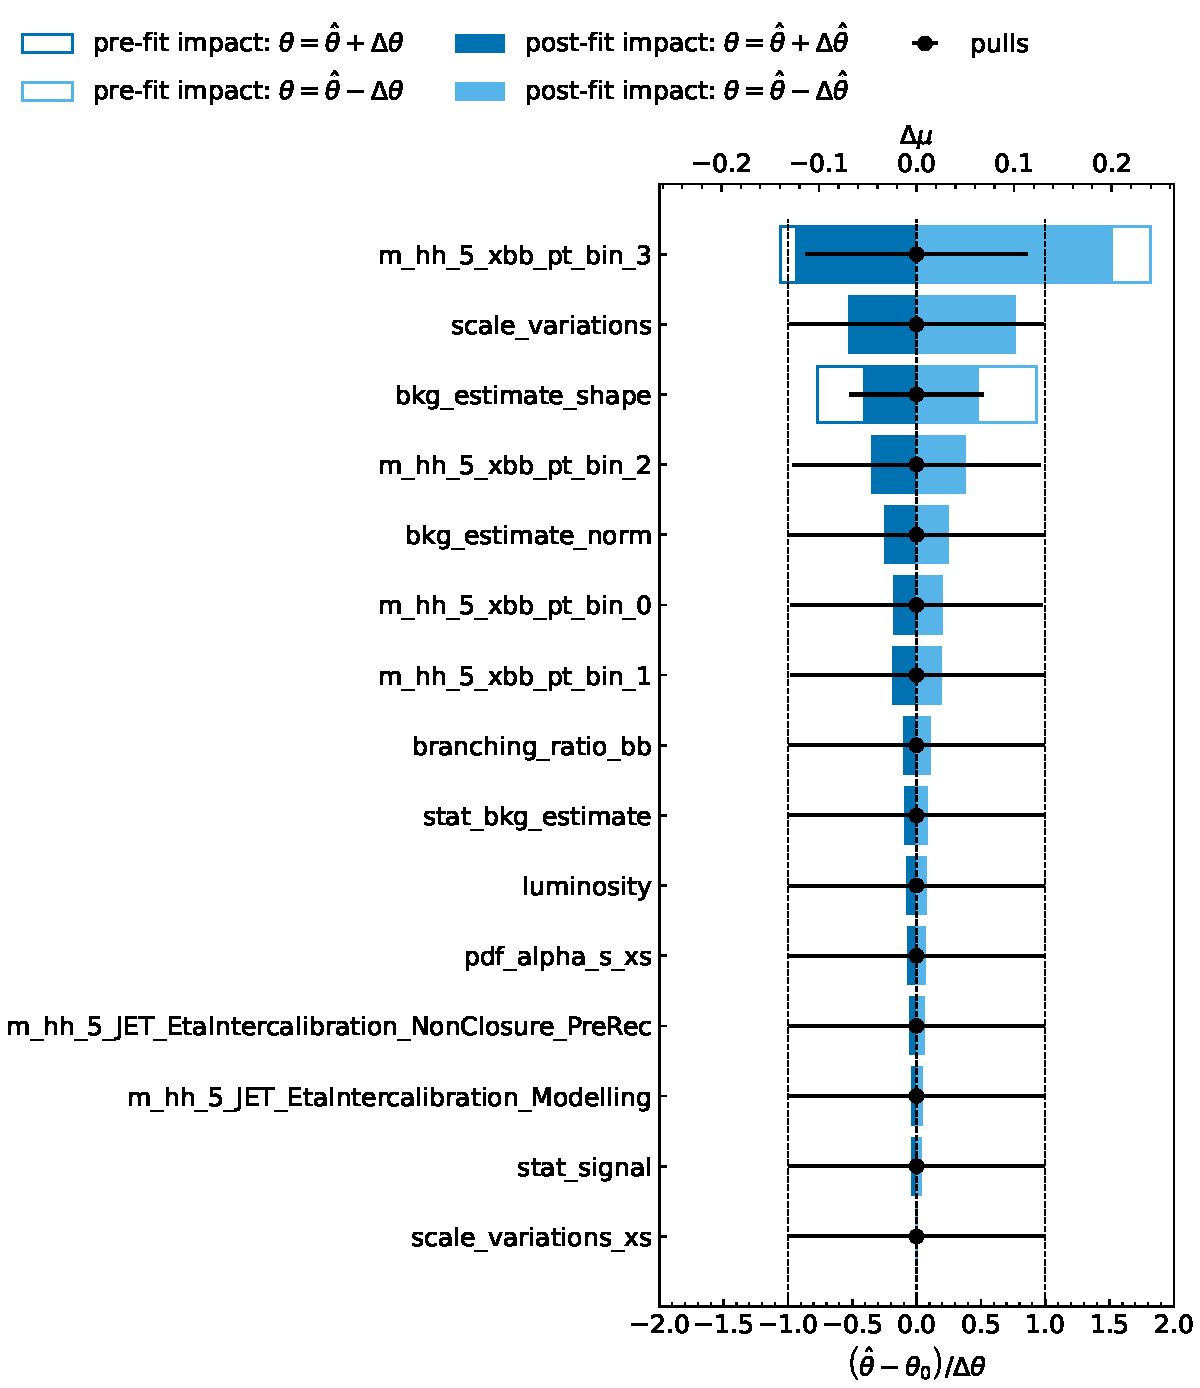
\includegraphics[width=1\textwidth]{neos_results/m_hh_5_full_sys_ranking.pdf}
    \caption[]{\red{redo, not all uncertainties, but to illustrate}
        Nuisance parameter impact ranking ordered by their post-fit impact on the signal strength $\Delta\mu$ on the upper axis for an invariant Higgs Pair mass fit \mhh{}. The impact of a nuisance parameter $\Theta$ is assessed by performing four fits. In each fit, a nuisance parameter is fixed to its nominal best fit value $\hat{\Theta}$ plus a given nuisance parameter uncertainty $\Delta\Theta$ and computes the difference of the resulting $\mu_\text{fit}$ from this fit with the nominal best fitted value $\Delta\mu=\hat{\mu} - \mu_\text{fit}$. This is repeated for pre-fit $\pm\Delta\Theta$ and post-fit $\pm\Delta\hat{\Theta}$ uncertainties of $\Theta$. The lower axis and the black points represent the pull for each nuisance paramter, calculated as the difference between the best-fit value and the nominal pre-fit $(\hat{\Theta} - \Theta_0)$, divided by its variance $\Delta\Theta$ for the parameter $\Theta$. If the model is accurate, the expected value of each pull should be zero, with a variance of one, given a sufficiently large sample size. In this asymptotic limit the test statistic is computed from the sum of pulls and follows a $\chi^2$ distribution if the model is correct. Thus, pulls serve as goodness-of-fit quantities. }
    \label{fig:m_hh_full_sys_ranking}
\end{figure}

\section{Training}

Figure \ref{fig:training_metrics_validation} presents the training loss and Asimov significance per eoch and as well histograms of the final model evaluated on the samples from table \ref{tab:neos-samples} for both the \ac{bce}-trained \ac{nn} and the neos \ac{nn}. While the loss function for the classifier converges for the validation dataset at about epoch 400 the cls loss evaluation shows strong signs of overfitting starting at epoch $\sim$200 \red{check 1e4/new trainings, so not necesarily final the next words} and thus the \ac{nn} from epoch 185 is chosen \ac{bce choice is 993}. The score of the \ac{bce}-trained \ac{nn} displays the typical feature of a classifier separation with most of the background in the lowest bin and falling event counts to larger values. When evaluated on signal samples the behavior is opposed. The largest impact of uncertainties on the signal is in the last bin. A different behavior can be observed in the histogram of the \ac{neos} approach. The signal sample is more spread over all bins and since a maximum likelihood fit exhibits a mirror symmetry for given histograms a spontaneous breaking of this symmetry can give inverted labeling for the \ac{nn} score. Furthermore, the Asimov significance, as defined in equation \ref{eq:asimov-significance}, commonly used as a proxy for statistical testing during analysis optimization, shows no clear correlation with the \ac{bce}-trained \ac{nn}. In contrast, it anti-correlates with the \ac{neos} loss function, hinting at a potential advantage of the neos approach.

\red{bkg estimation input is clipped, also describe in methods}

cut runter korrespondiert eig zu weniger daten während training --> cuts rausfahren
eig gut ohne cuts zuerst trainieren dann, model nehmen und cut optimieren...  evtl macht das das lange trianing

man kann alles zs machen, aber eig in zwei steps

show mit giffer, das up down sehr hin und her springt --> training mit guten cut
mit learning rate weiter runter gehen, wenn das so sprint?
bkg uncertainty film

\begin{figure}
    \centering
    \subfigure[]{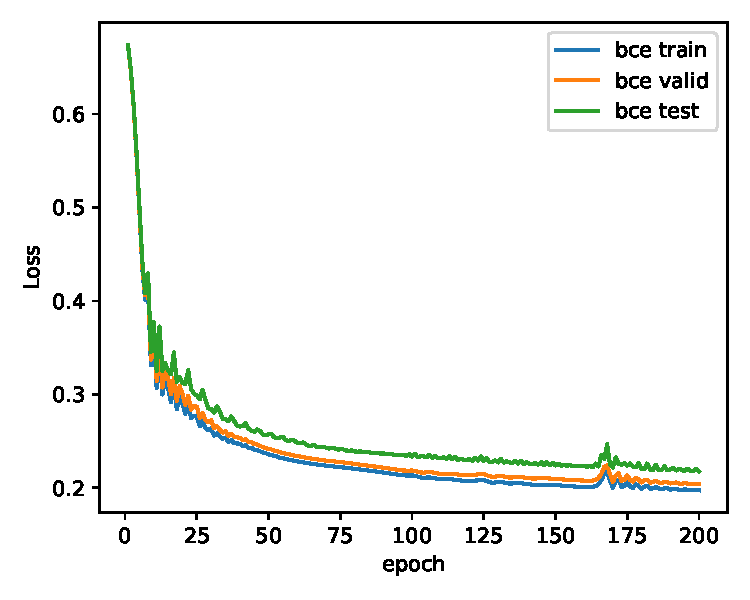
\includegraphics[width=.45\textwidth]{tomatos_bce_5_1000/bce.pdf}}
    \subfigure[]{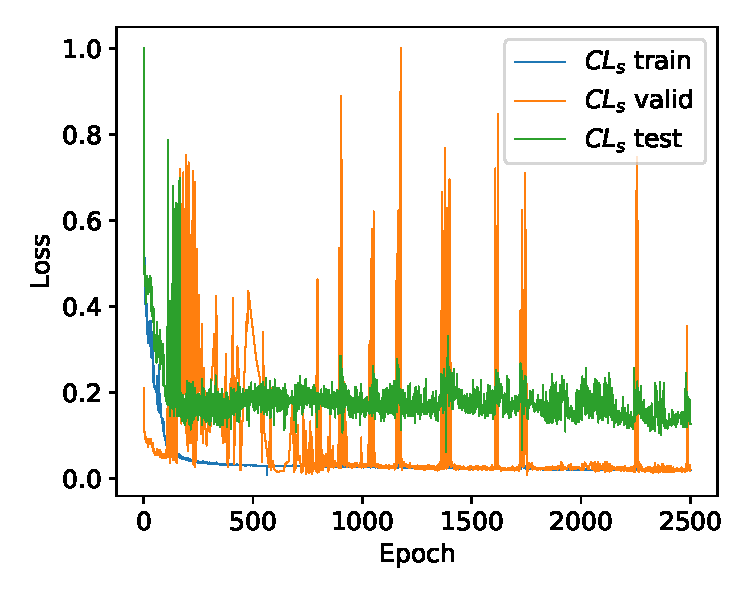
\includegraphics[width=.45\textwidth]{tomatos_cls_5_1000_unbound_shapesys/cls.pdf}} \label{fig:neos_validation_loss}\\
    \subfigure[]{\includegraphics[width=.45\textwidth]{tomatos_bce_5_1000/hist.pdf}}
    \subfigure[]{\includegraphics[width=.45\textwidth]{tomatos_cls_5_400_unbound_shapesys/hist.pdf}} \\
    \subfigure[]{\includegraphics[width=.45\textwidth]{tomatos_bce_5_1000/Z_A.pdf}}
    \subfigure[]{\includegraphics[width=.45\textwidth]{tomatos_cls_5_1000_unbound_shapesys/Z_A.pdf}} \\
    \caption[]{\textbf{(Left Column)} \ac{nn} trained with a \ac{bce} loss function. \textbf{(Right Coloumn)} \ac{nn} trained with \ac{neos}.  \textbf{(Top To bottom)}: Loss function evaluated on training, validation and test dataset per training epoch, histogrammed \ac{nn} score for samples used in the training and Asimov significance. \red{redo all plots, significance wrong, make sure sys are same} }
    \label{fig:training_metrics_validation}
\end{figure}



\section{Performance Comparison}
After training the \acp{nn} they are evaluated alongside an $\mhh$ fit without the use of any \ac{neos} methods to determine limits on the boosted \ac{vbf} $HH\rightarrow4b$ cross-section with the \textit{cabinetry} fitting framework \citep{cranmer_2021_4627038}. Hence, the event selection, application of cuts or the creation of histograms are applied traditionally.

\begin{figure}
    \centering
    \subfigure[]{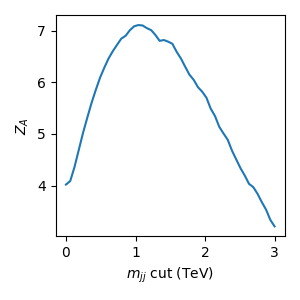
\includegraphics[width=.3\textwidth]{s_b_optimization/s_b_optimization_m_hh_5_m_jj}}
    \subfigure[]{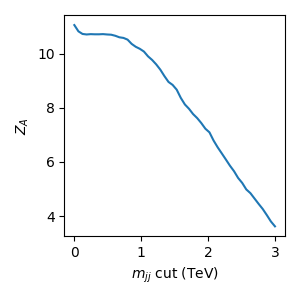
\includegraphics[width=.3\textwidth]{s_b_optimization/s_b_optimization_tomatos_bce_5_1000_m_jj}}
    \subfigure[]{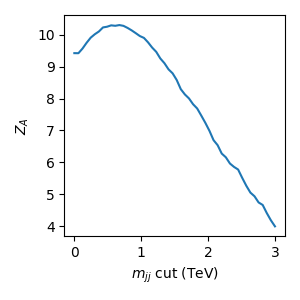
\includegraphics[width=.3\textwidth]{s_b_optimization/s_b_optimization_tomatos_cls_5_400_unbound_shapesys_m_jj}}\\
    \subfigure[]{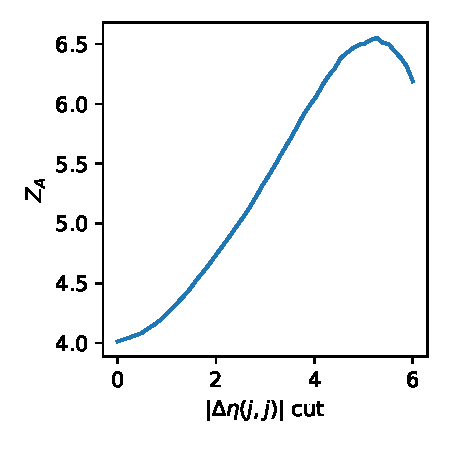
\includegraphics[width=.3\textwidth]{s_b_optimization/s_b_optimization_m_hh_5_eta_jj}}
    \subfigure[]{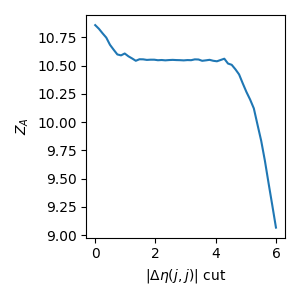
\includegraphics[width=.3\textwidth]{s_b_optimization/s_b_optimization_tomatos_bce_5_1000_eta_jj}}
    \subfigure[]{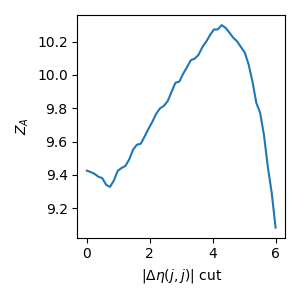
\includegraphics[width=.3\textwidth]{s_b_optimization/s_b_optimization_tomatos_cls_5_400_unbound_shapesys_eta_jj}}
    \caption[]{Columns left to right: $\mhh$, \ac{bce}-trained \ac{nn}, \ac{neos}-trained \ac{nn}: Asimov Significances after applying a cut on \textbf{(a)-(c)} on the invariant mass $m_{jj}$ and the pseudorapidity separation \textbf{(d)-(f)} $|\Delta\eta(j,j)|$ of the \ac{vbf} jets.}
    \label{fig:cut_scan}
\end{figure}

To determine the $m_{jj}$ and $|\Delta\eta(j,j)|$ cuts on the \ac{vbf} jets, cuts are scanned and the resulting histogram is evaluated on the Asimov significance for the three variables. Figure \ref{fig:cut_scan} the results of this procedure depending on the cuts and table \ref{tab:z_a_cuts} displays the derived cuts from maximizing the Asimov significance. Cuts found by the \ac{neos} optimization as explained in \ref{sec:neos_training} are shown in figure \ref{fig:neos_cuts}. These also potentially explain the shape of the validation loss for the \ac{neos} training as of figure \ref{fig:neos_validation_loss}. Even though the introduction of new data is always beneficial in training, overtraining starts around epoch 200 and worsens until epoch 400 which is where the cuts merely change. Upon introducing more data by further loosening the cuts around epoch 400 the validation also decreases again until at epoch 600 where $m_{jj}$ plateaus again. However the \ac{nn} is potentially already in a local overtrained minimum showing no signs of further improvement and the training becomes unstable. \red{This is further investigated in chapter \ref{ch:hh4b-results}.}

\begin{figure}
    \centering
    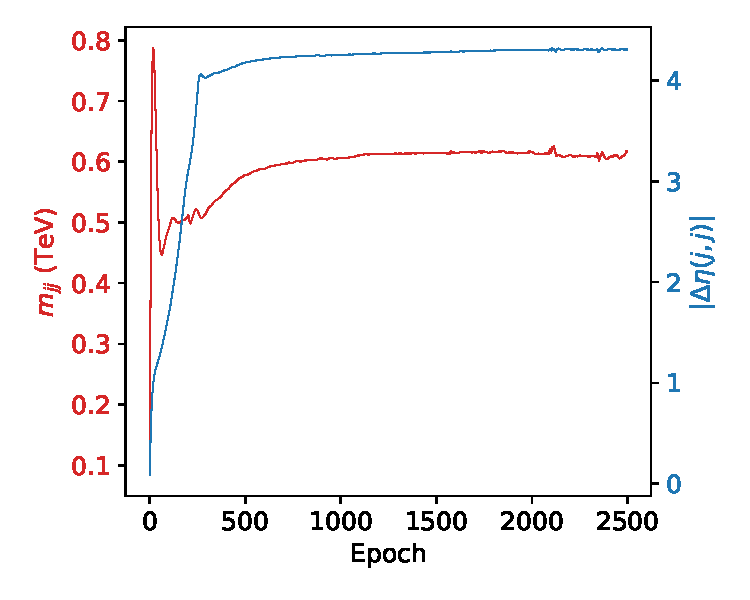
\includegraphics[width=.6\textwidth]{tomatos_cls_5_1000_unbound_shapesys/cuts}
    \caption[]{Optimized \ac{neos} cuts per epoch for the invariant mass $m_{jj}$ and the pseudorapidity difference $|\Delta\eta(j,j)|$ of the two \ac{vbf} jets.}
    \label{fig:neos_cuts}
\end{figure}
\begin{table}[htbp]\label{tab:z_a_cuts}
    \centering
    \caption{Optimized cuts for \mhh and the trained \acp{nn} from the maximized Asimov significances shown in figure \ref{fig:cut_scan} and the cuts found by the \ac{neos} optimization in epoch 185 of figure \ref{fig:neos_cuts}.}
    \begin{tabular}{c|c|c}
                                  & $m_{jj}$ (GeV) & $|\Delta\eta(j,j)|$ \\\hline
        \mhh                      & >1041          & >5.27               \\
        \ac{bce}-trained \ac{nn}  & >0             & >0                  \\
        \ac{neos}-trained \ac{nn} & >673           & >4.29               \\ \hline
        \ac{neos} (epoch 185)     & >481           & >1.45               \\
    \end{tabular}
\end{table}

All models use the same methods for the background uncertainty estimation described in \ref{sec:bkg_uncertainties}. Uncertainties used for the fitting are shown in figure \ref{fig:neos_validation_uncertaintes_1} and \ref{fig:neos_validation_uncertaintes_2}. \ac{ggf} signal uncertainties are omitted here as the difference of adding the \ac{ggf} signal to the fitting procedure has a \qty{1}{\percent}(\qty{0.5}{\percent}) impact on the cross-section limits when using the \ac{sm}($\ktwov=0$) \ac{vbf} signal in the maximum likelihood fit.

\begin{figure}
    \centering
    \subfigure[]{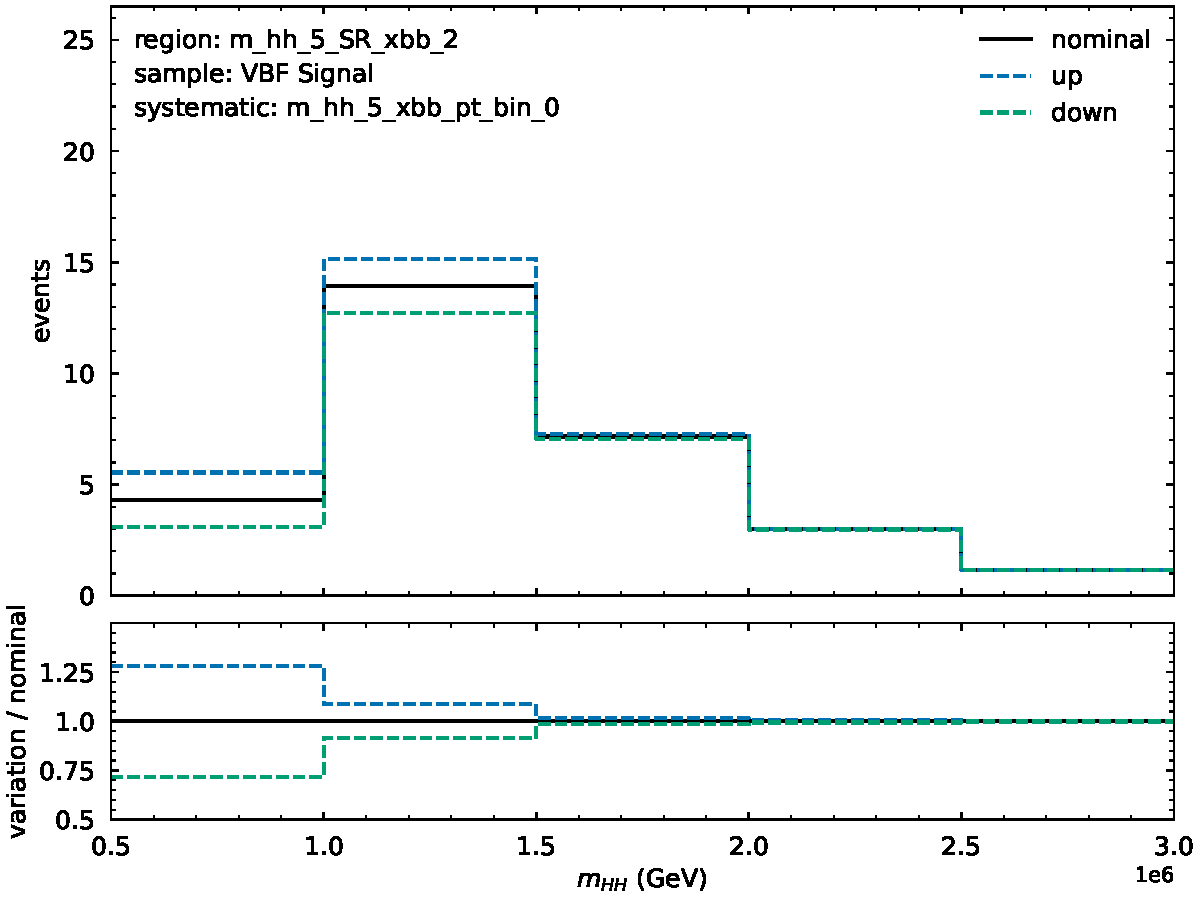
\includegraphics[width=.3\textwidth]{neos_results/m_hh_5_l1cvv0cv1/figures/templates/m_hh_5_SR_xbb_2_VBF-Signal_m_hh_5_xbb_pt_bin_0.pdf}}
    \subfigure[]{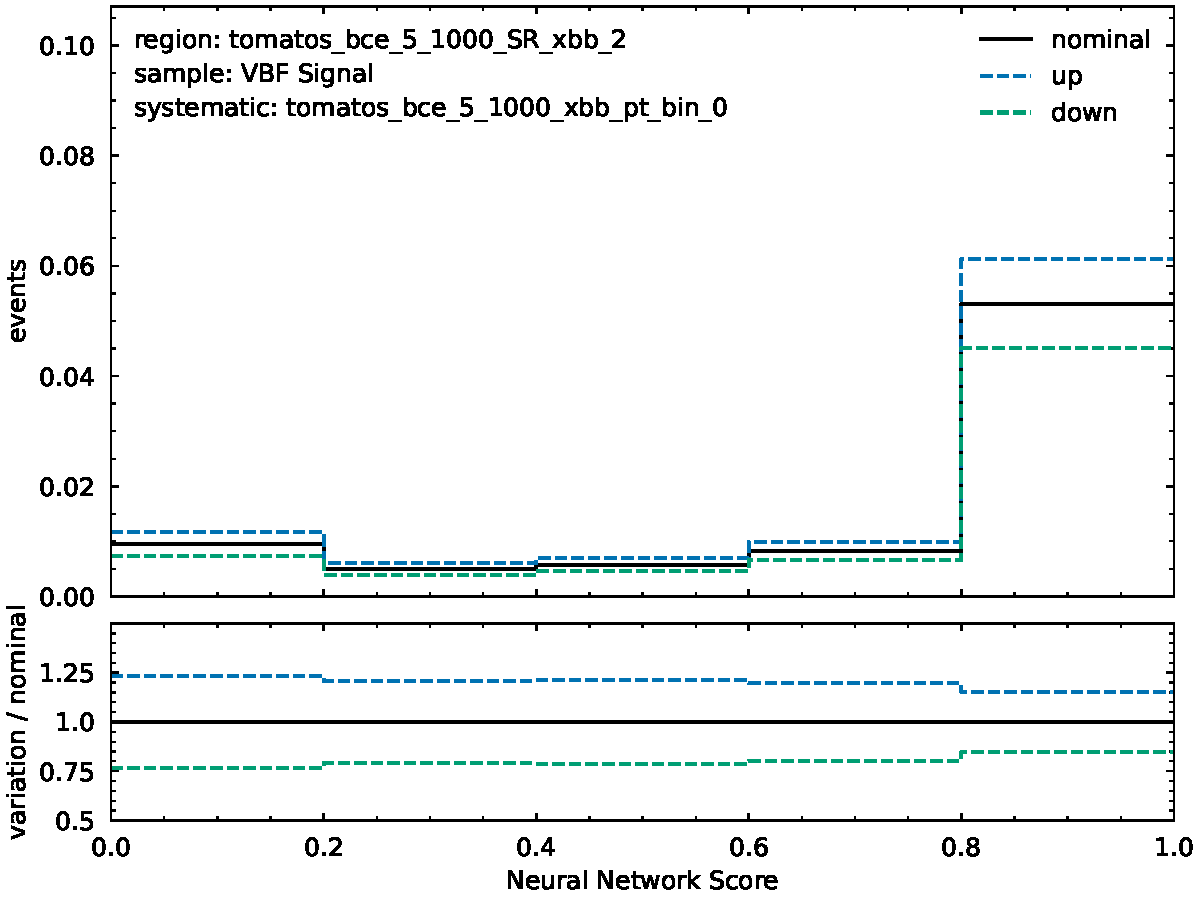
\includegraphics[width=.3\textwidth]{neos_results/tomatos_bce_5_1000_l1cvv0cv1/figures/templates/tomatos_bce_5_1000_SR_xbb_2_VBF-Signal_tomatos_bce_5_1000_xbb_pt_bin_0.pdf}}
    \subfigure[]{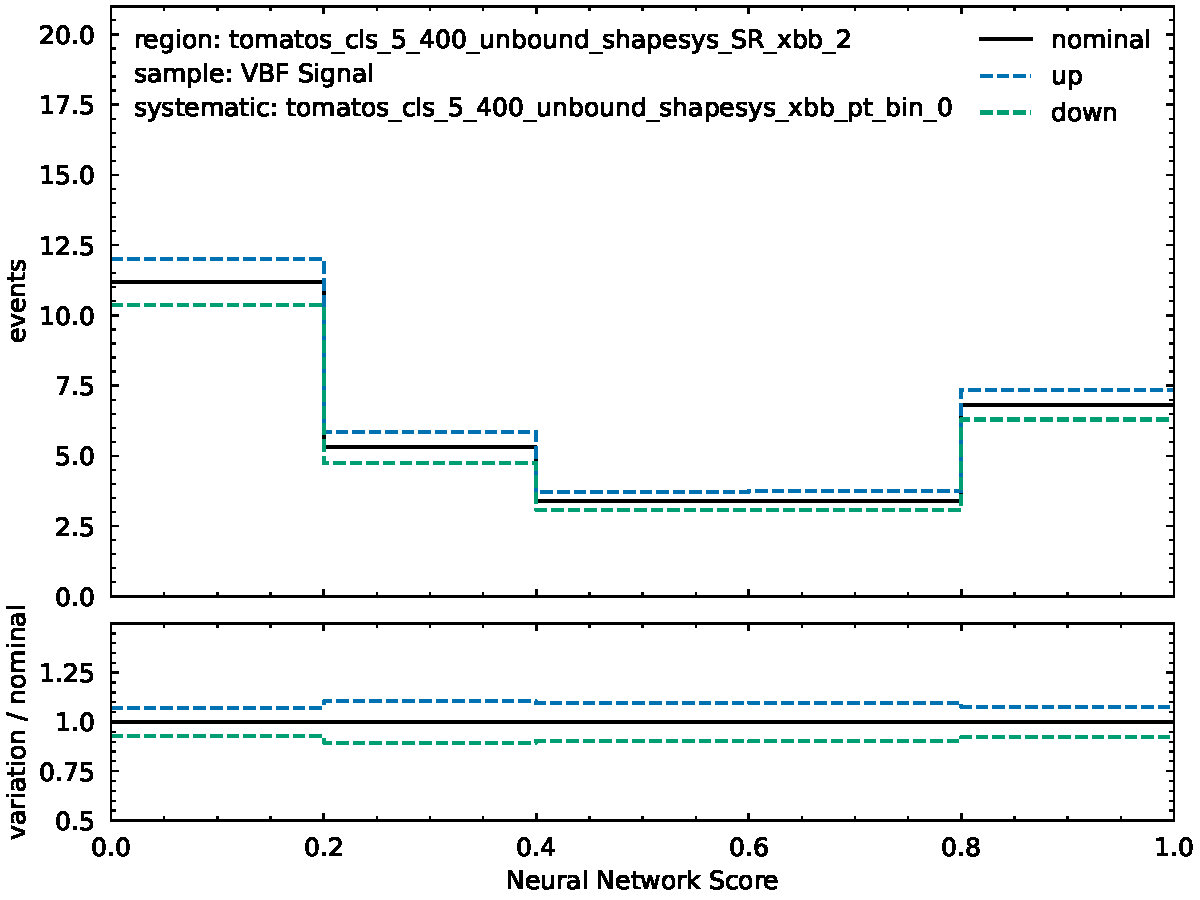
\includegraphics[width=.3\textwidth]{neos_results/tomatos_cls_5_400_unbound_shapesys_l1cvv0cv1/figures/templates/tomatos_cls_5_400_unbound_shapesys_SR_xbb_2_VBF-Signal_tomatos_cls_5_400_unbound_shapesys_xbb_pt_bin_0.pdf}} \\
    \subfigure[]{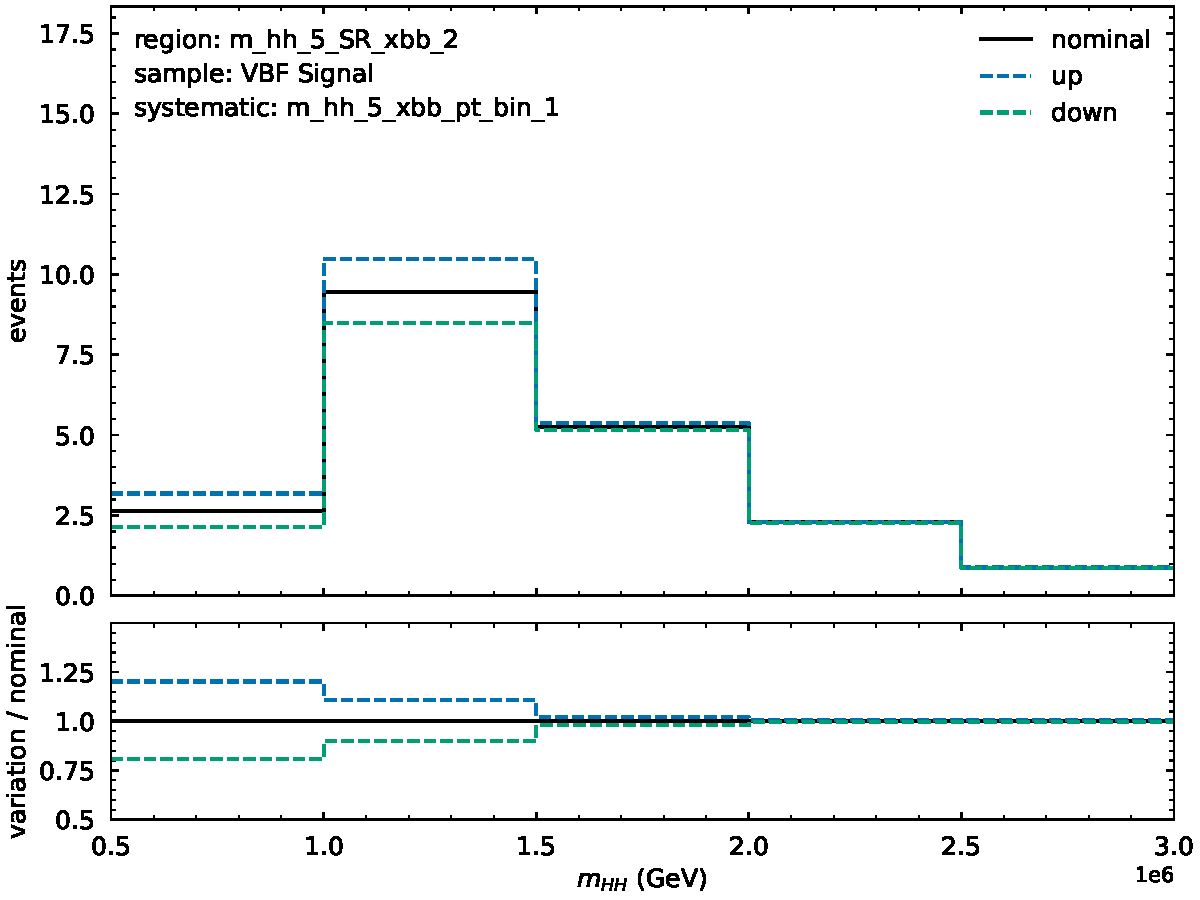
\includegraphics[width=.3\textwidth]{neos_results/m_hh_5_l1cvv0cv1/figures/templates/m_hh_5_SR_xbb_2_VBF-Signal_m_hh_5_xbb_pt_bin_1.pdf}}
    \subfigure[]{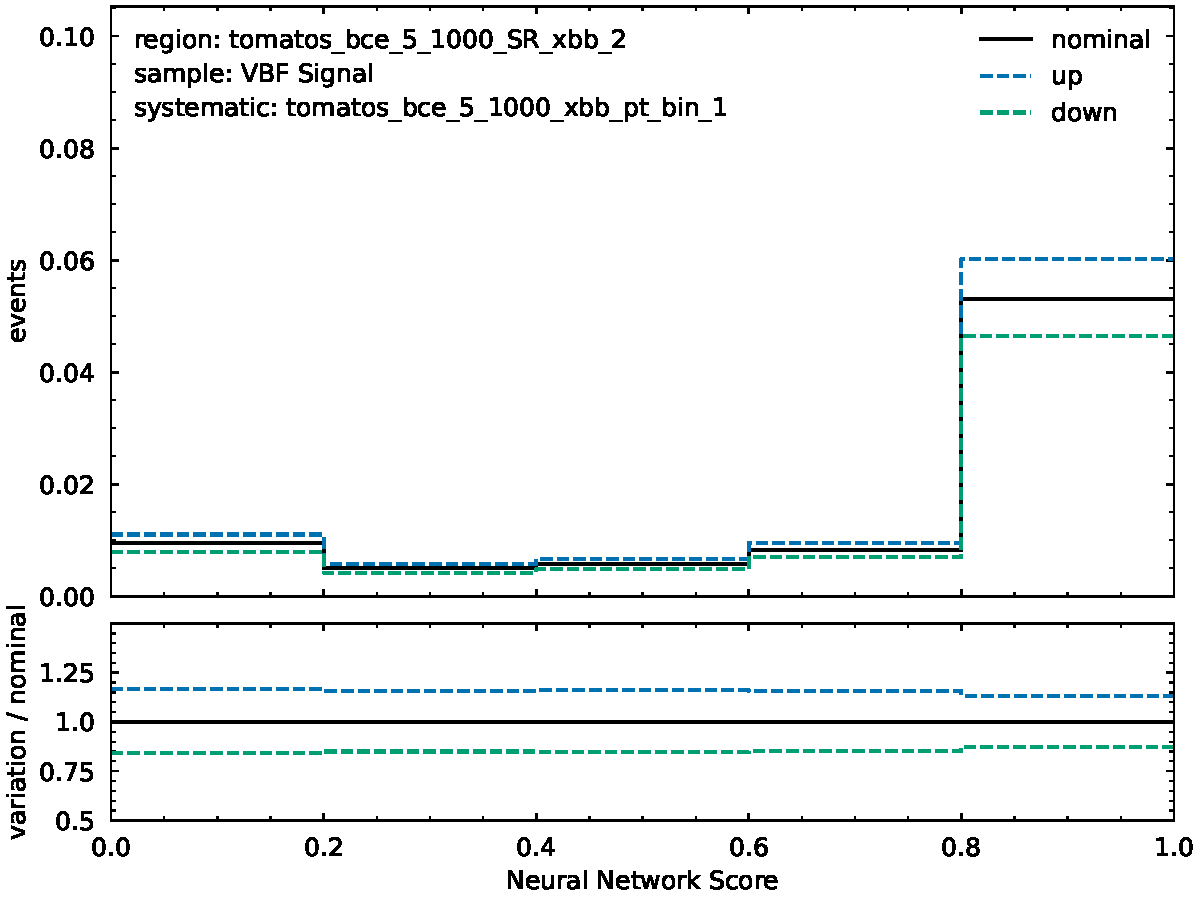
\includegraphics[width=.3\textwidth]{neos_results/tomatos_bce_5_1000_l1cvv0cv1/figures/templates/tomatos_bce_5_1000_SR_xbb_2_VBF-Signal_tomatos_bce_5_1000_xbb_pt_bin_1.pdf}}
    \subfigure[]{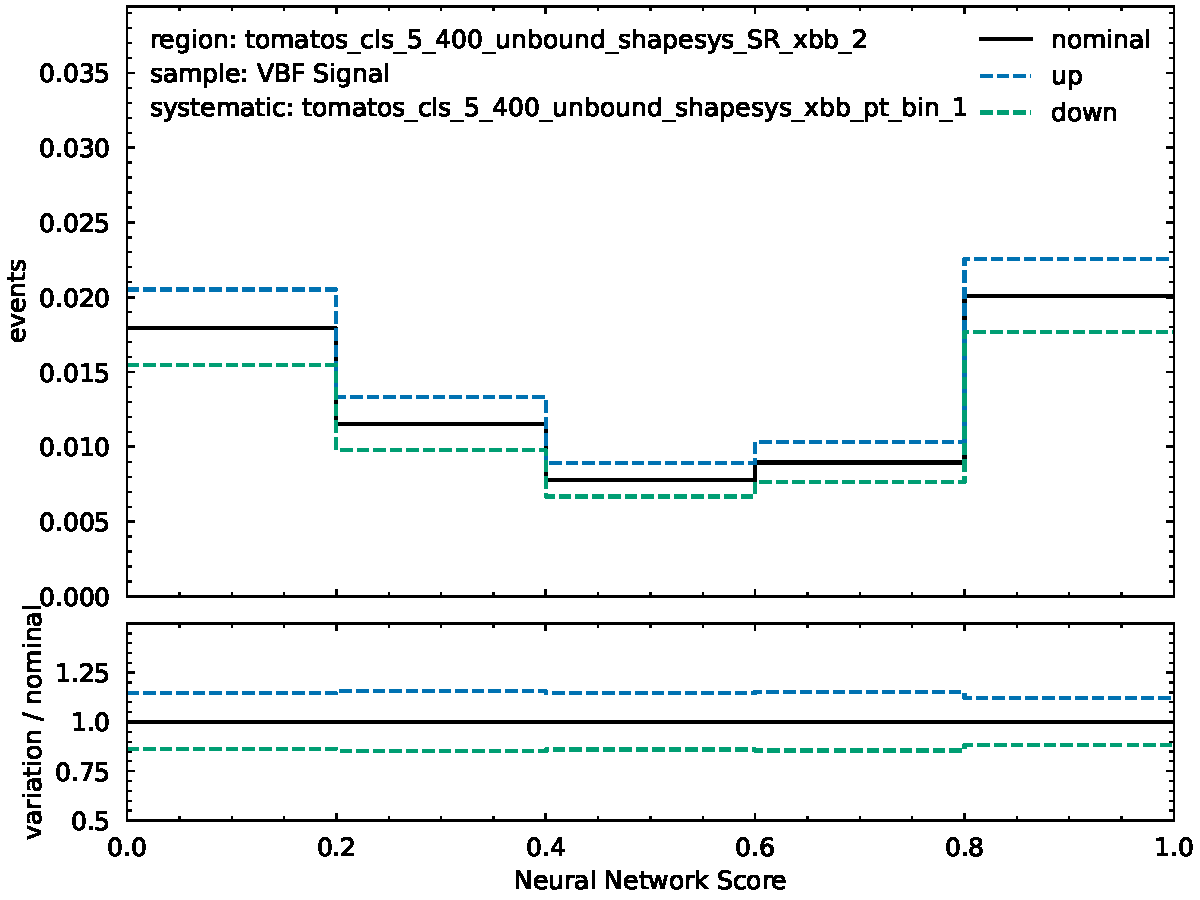
\includegraphics[width=.3\textwidth]{neos_results/tomatos_cls_5_400_unbound_shapesys_l1cvv0cv1/figures/templates/tomatos_cls_5_400_unbound_shapesys_SR_xbb_2_VBF-Signal_tomatos_cls_5_400_unbound_shapesys_xbb_pt_bin_1.pdf}} \\
    \subfigure[]{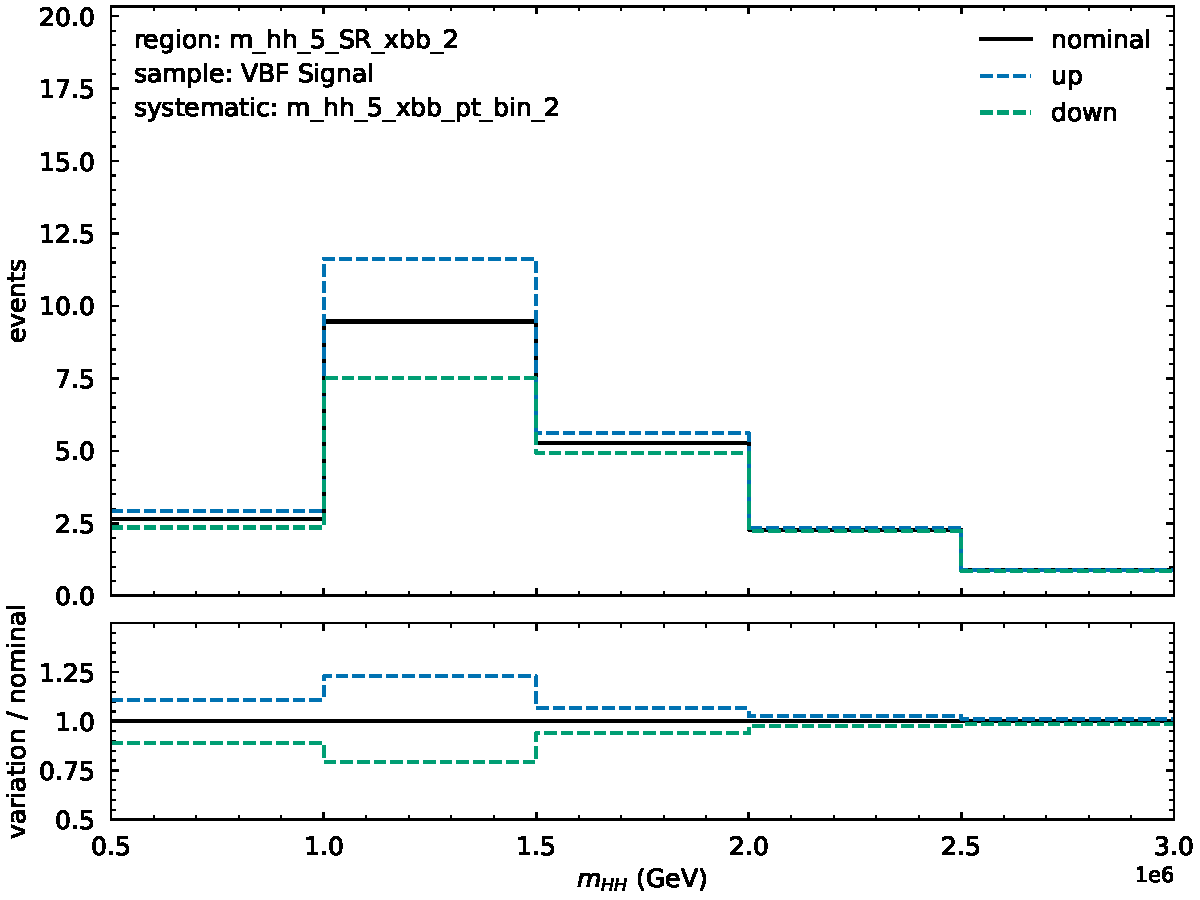
\includegraphics[width=.3\textwidth]{neos_results/m_hh_5_l1cvv0cv1/figures/templates/m_hh_5_SR_xbb_2_VBF-Signal_m_hh_5_xbb_pt_bin_2.pdf}}
    \subfigure[]{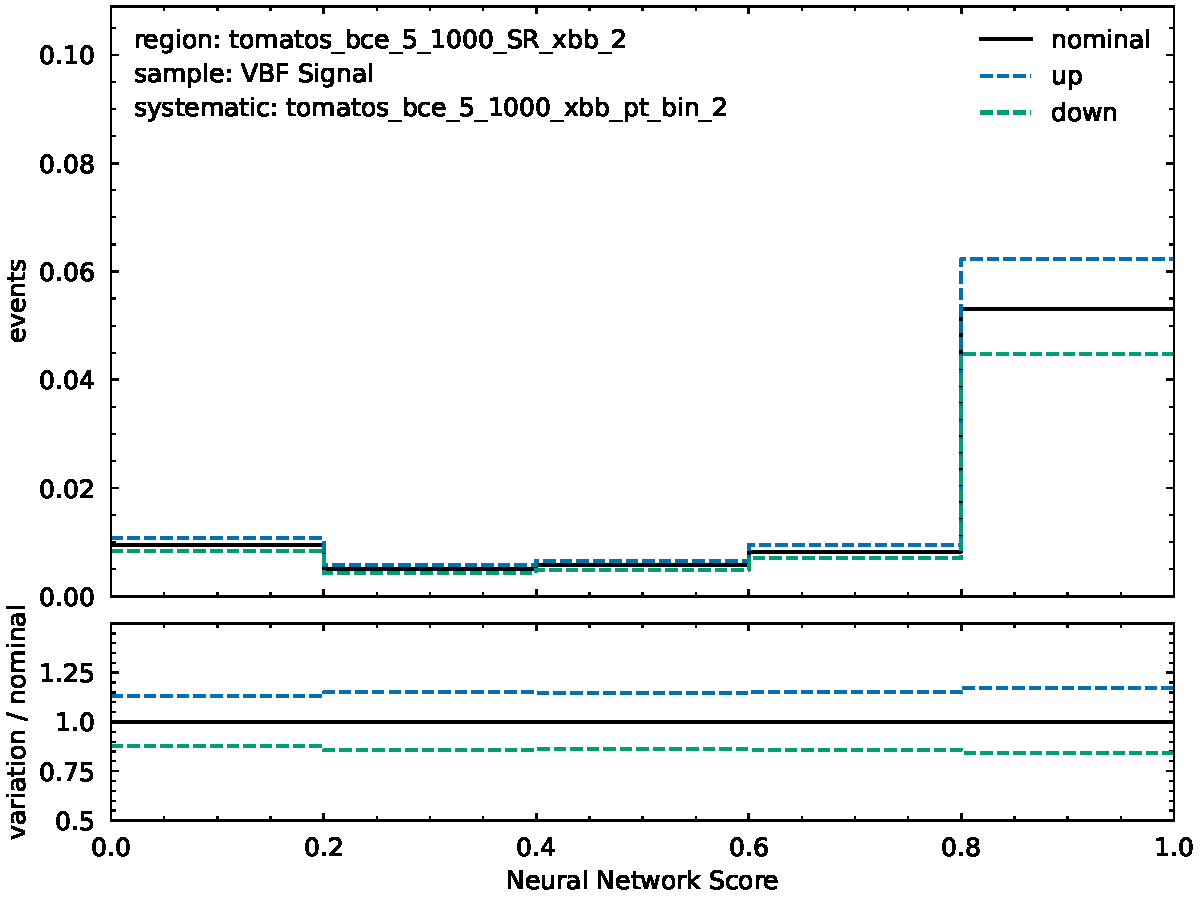
\includegraphics[width=.3\textwidth]{neos_results/tomatos_bce_5_1000_l1cvv0cv1/figures/templates/tomatos_bce_5_1000_SR_xbb_2_VBF-Signal_tomatos_bce_5_1000_xbb_pt_bin_2.pdf}}
    \subfigure[]{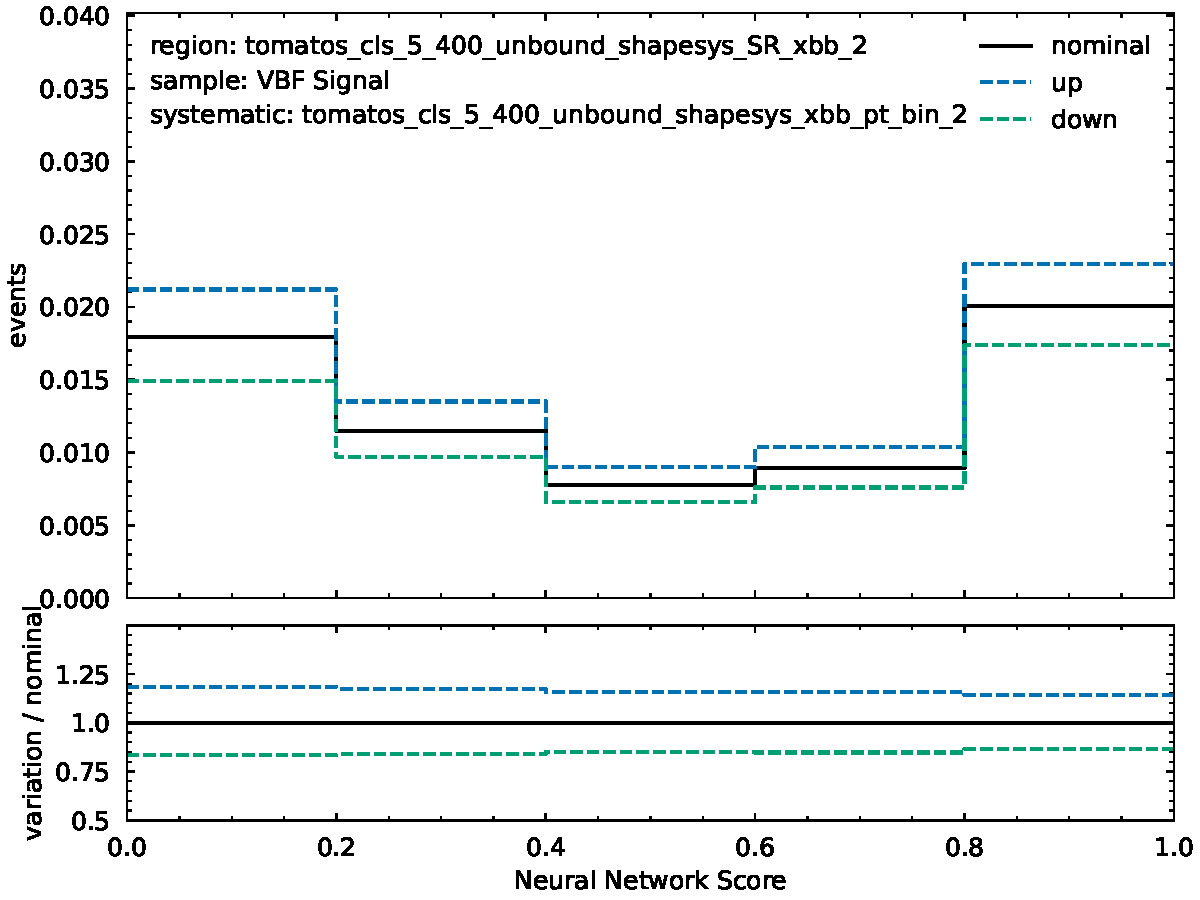
\includegraphics[width=.3\textwidth]{neos_results/tomatos_cls_5_400_unbound_shapesys_l1cvv0cv1/figures/templates/tomatos_cls_5_400_unbound_shapesys_SR_xbb_2_VBF-Signal_tomatos_cls_5_400_unbound_shapesys_xbb_pt_bin_2.pdf}} \\
    \subfigure[]{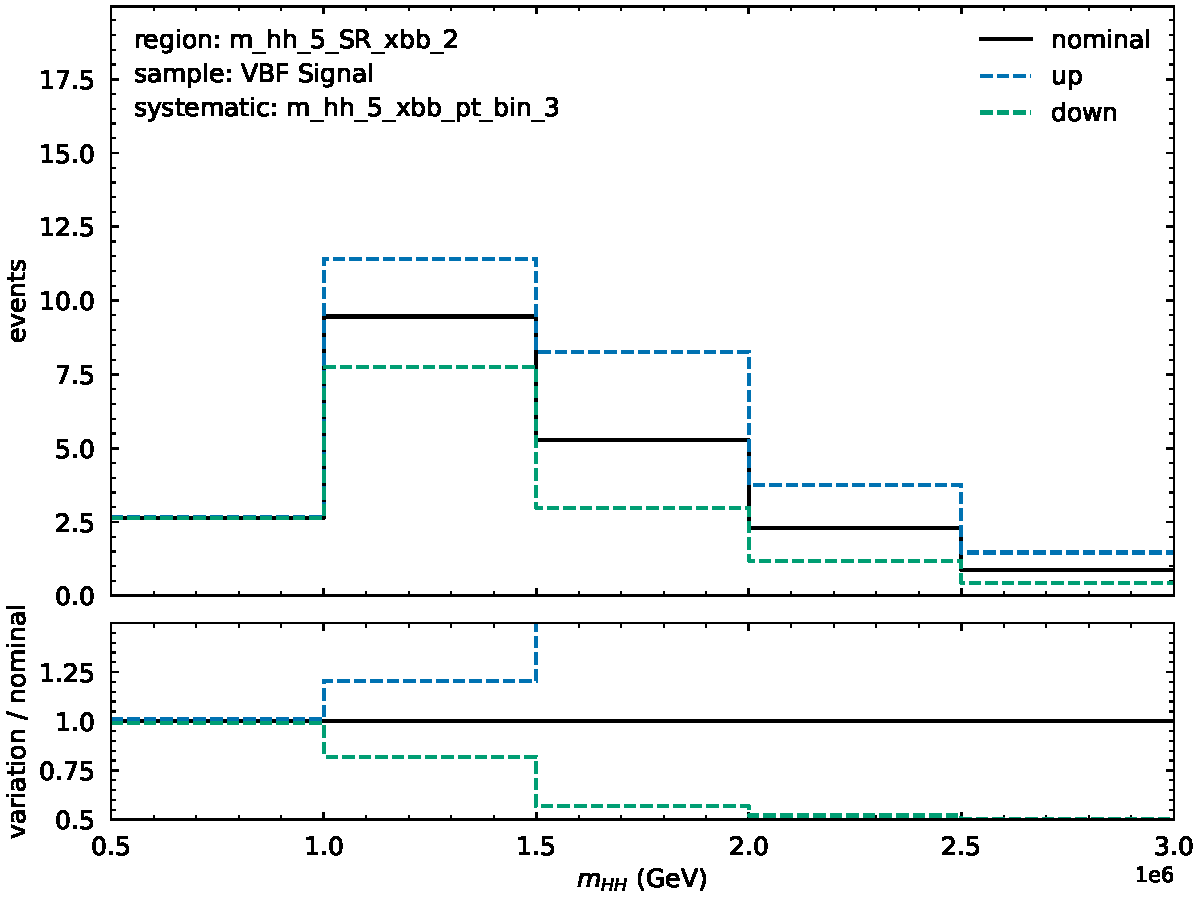
\includegraphics[width=.3\textwidth]{neos_results/m_hh_5_l1cvv0cv1/figures/templates/m_hh_5_SR_xbb_2_VBF-Signal_m_hh_5_xbb_pt_bin_3.pdf}}
    \subfigure[]{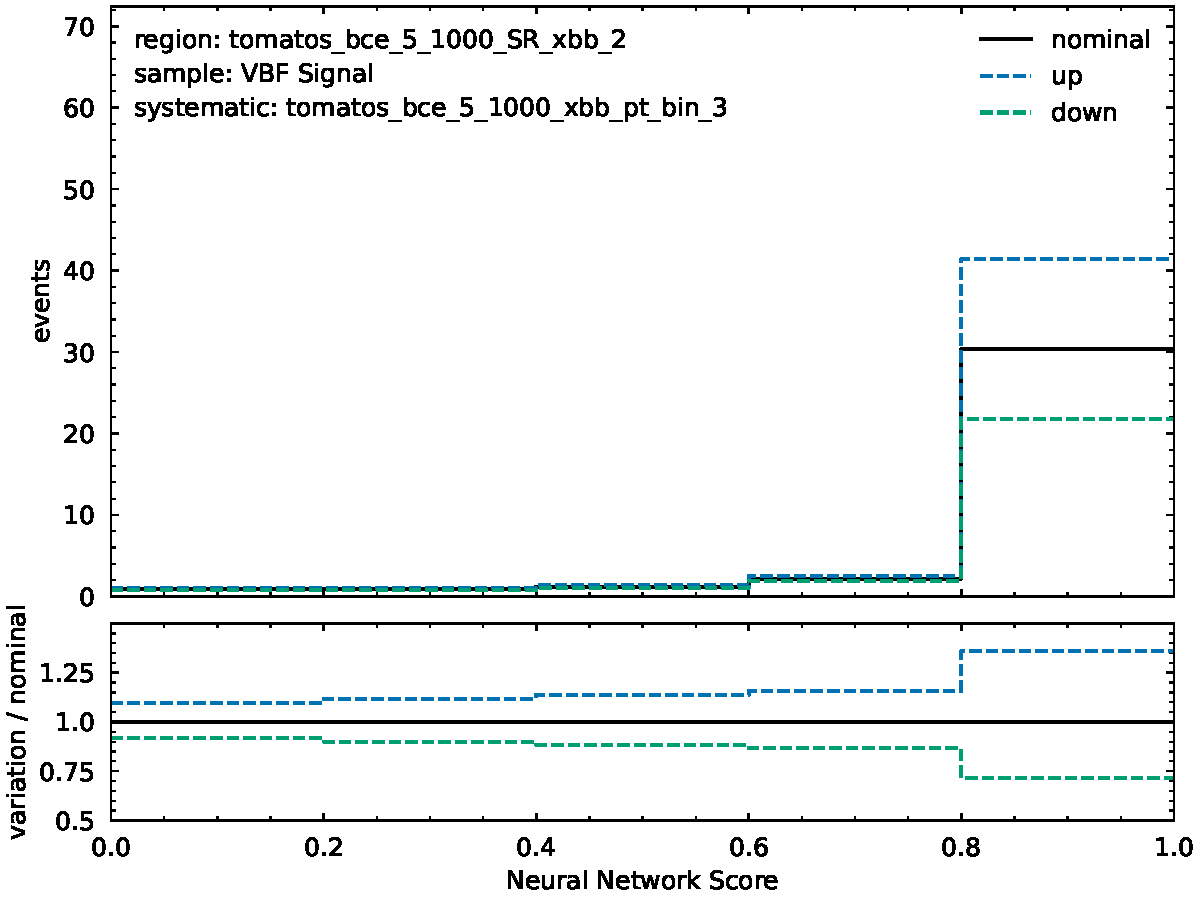
\includegraphics[width=.3\textwidth]{neos_results/tomatos_bce_5_1000_l1cvv0cv1/figures/templates/tomatos_bce_5_1000_SR_xbb_2_VBF-Signal_tomatos_bce_5_1000_xbb_pt_bin_3.pdf}}
    \subfigure[]{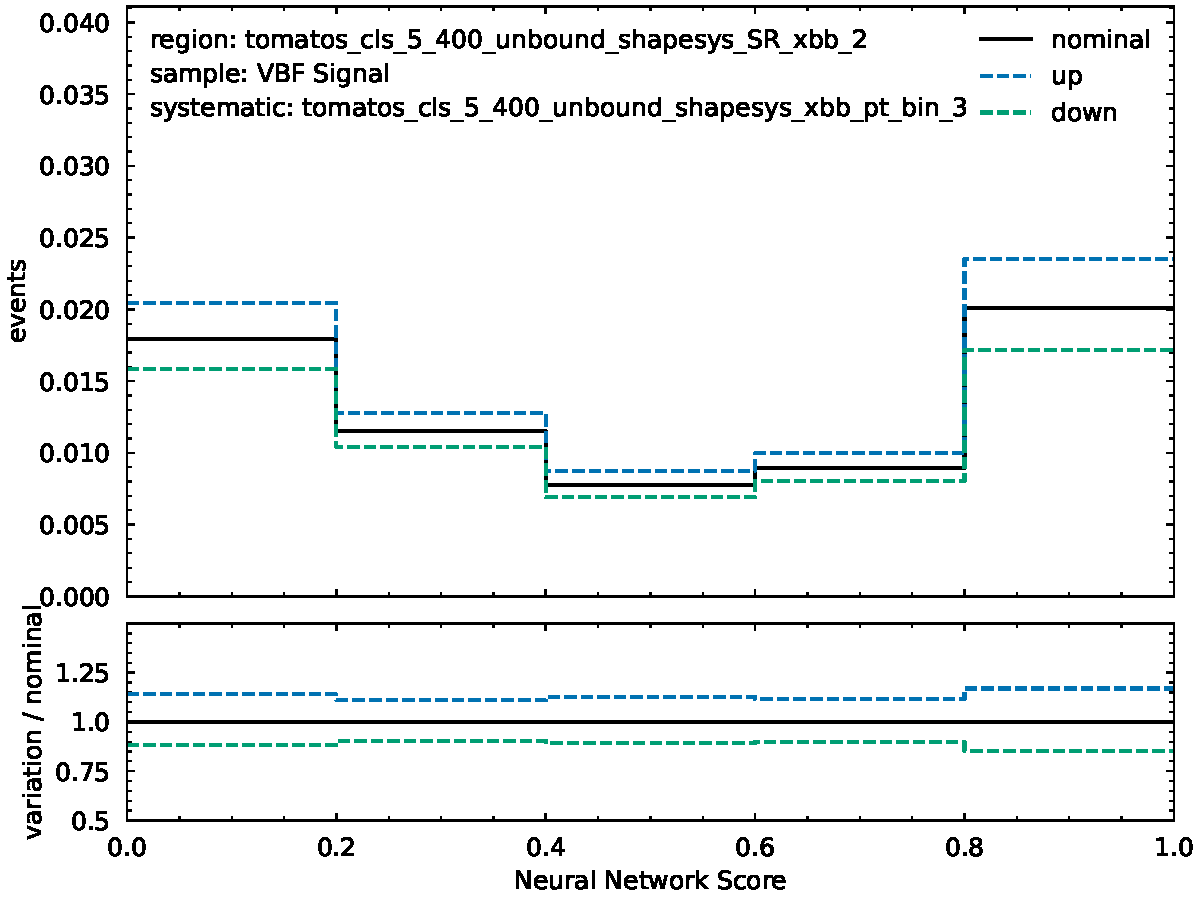
\includegraphics[width=.3\textwidth]{neos_results/tomatos_cls_5_400_unbound_shapesys_l1cvv0cv1/figures/templates/tomatos_cls_5_400_unbound_shapesys_SR_xbb_2_VBF-Signal_tomatos_cls_5_400_unbound_shapesys_xbb_pt_bin_3.pdf}} \\
    \caption[]{Uncertainties (1/2) for columns left to right: $\mhh$, \ac{bce}-trained \ac{nn}, \ac{neos}-trained \ac{nn}. Top to bottom: 30\% GN2X scale factor uncertainties for the four bins used in the calibration of the GN2X tagger as shown in figure \ref{fig:xbb_sf}.\red{increase labels}}
    \label{fig:neos_validation_uncertaintes_1}
\end{figure}
\begin{figure}
    \centering
    \subfigure[]{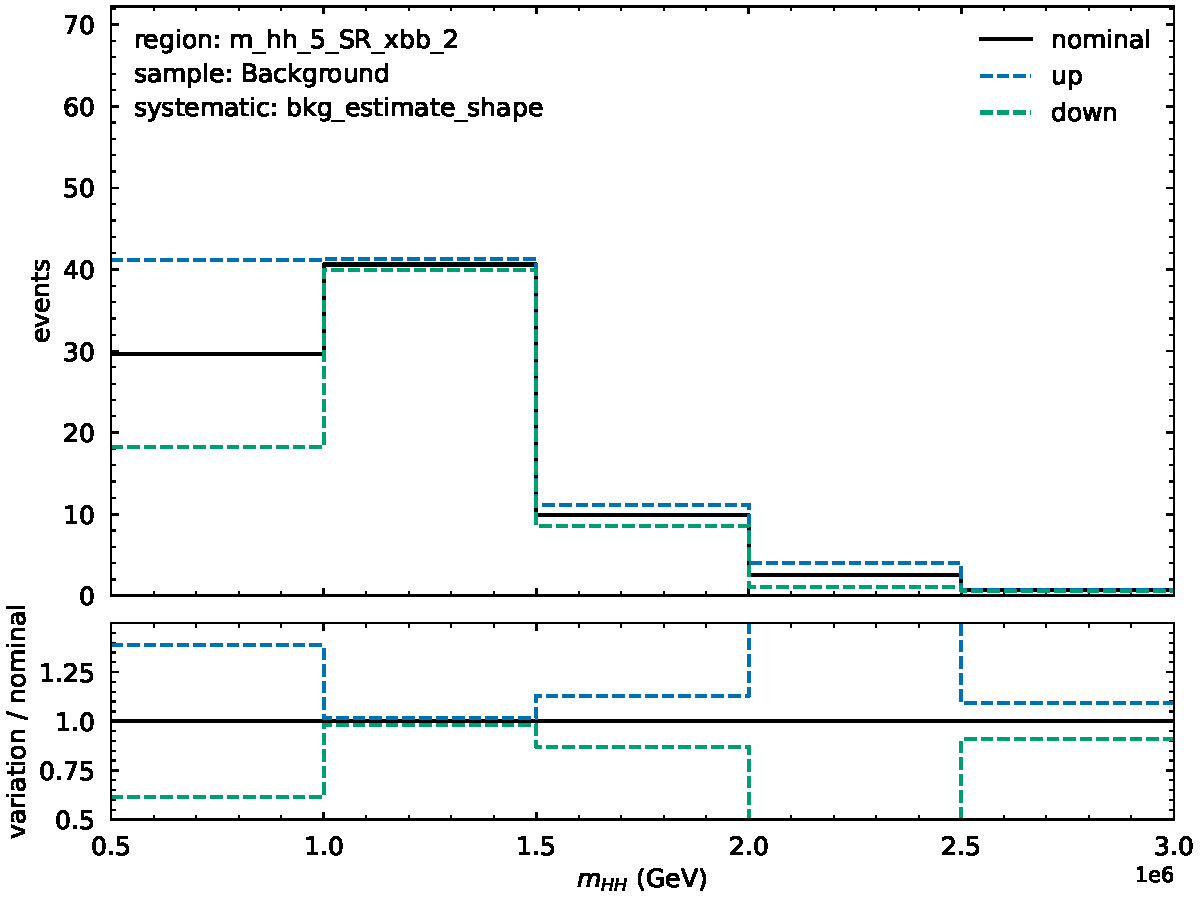
\includegraphics[width=.3\textwidth]{neos_results/m_hh_5_l1cvv0cv1/figures/templates/m_hh_5_SR_xbb_2_Background_bkg_estimate_shape.pdf}}    \subfigure[]{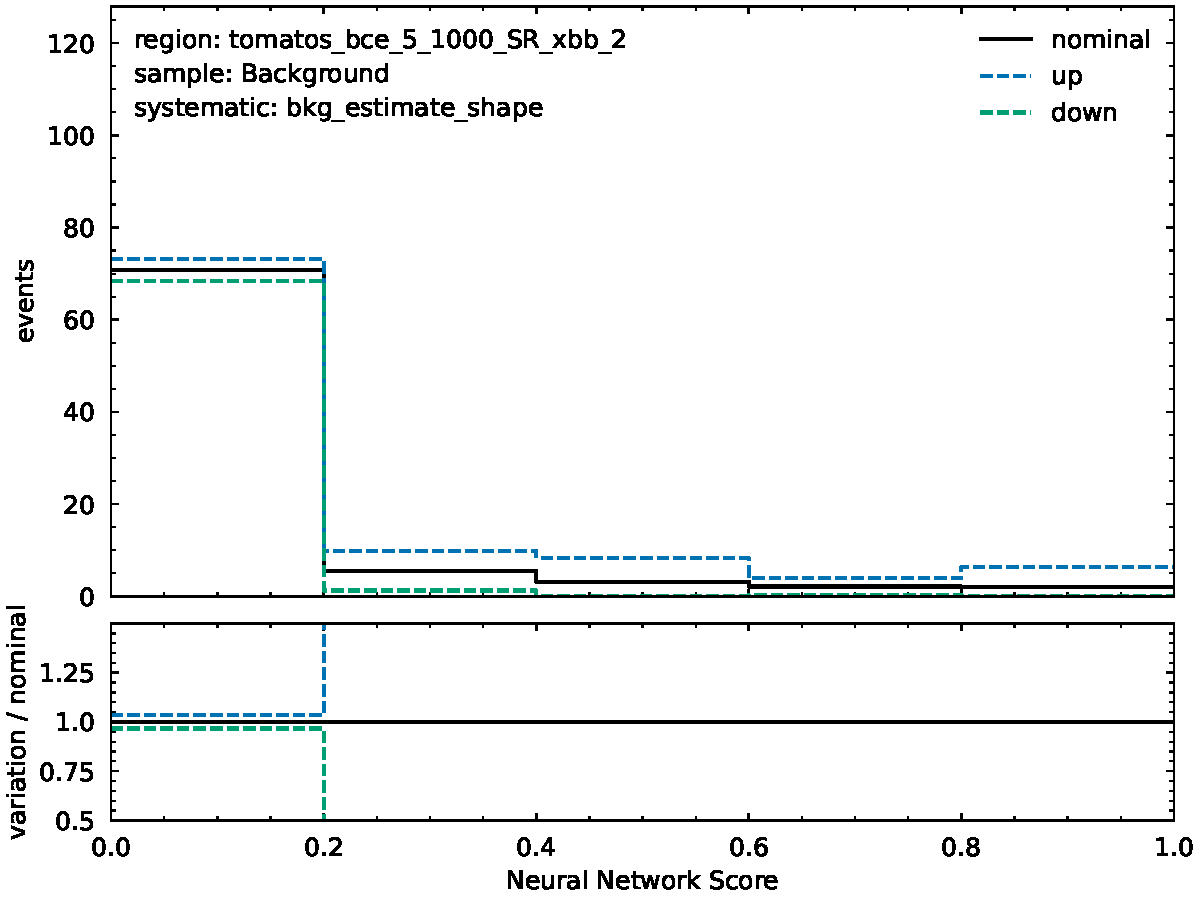
\includegraphics[width=.3\textwidth]{neos_results/tomatos_bce_5_1000_l1cvv0cv1/figures/templates/tomatos_bce_5_1000_SR_xbb_2_Background_bkg_estimate_shape.pdf}}
    \subfigure[]{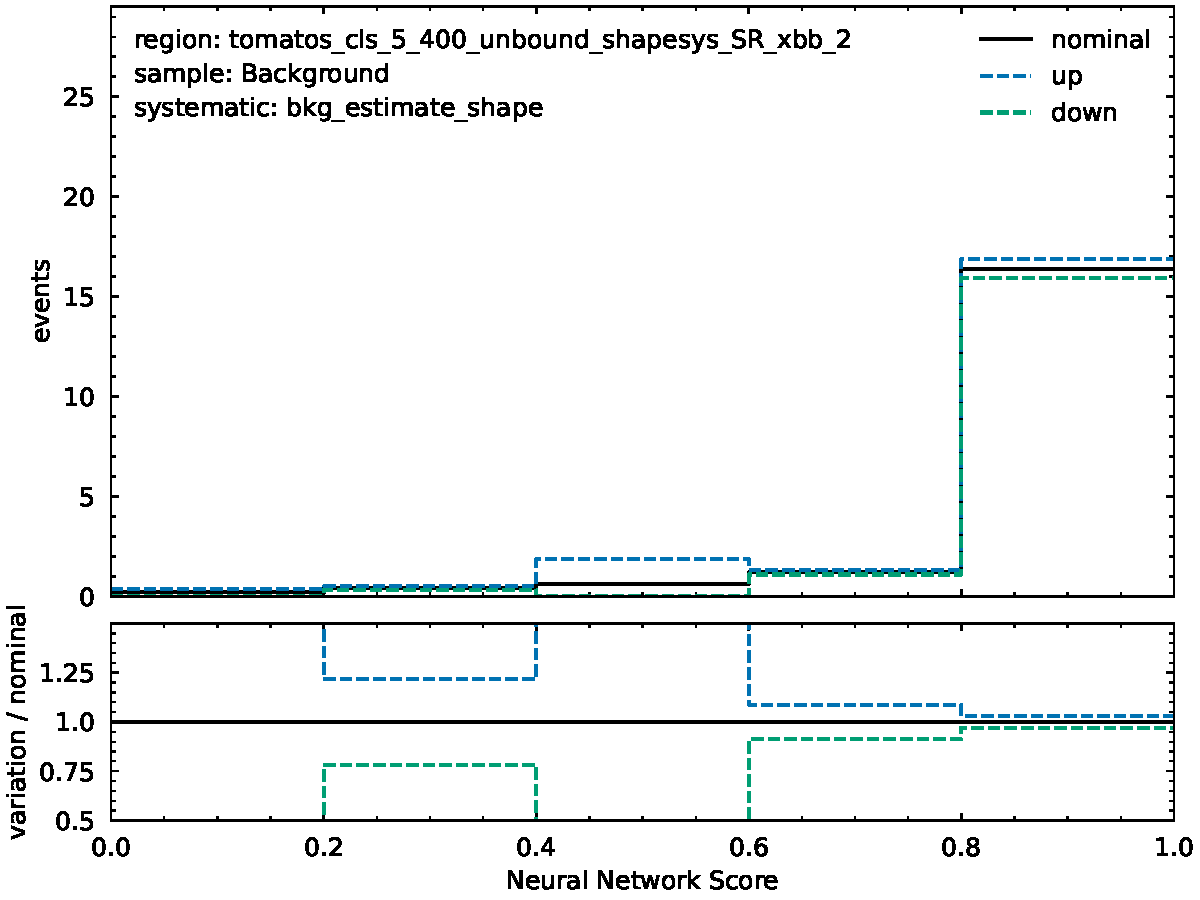
\includegraphics[width=.3\textwidth]{neos_results/tomatos_cls_5_400_unbound_shapesys_l1cvv0cv1/figures/templates/tomatos_cls_5_400_unbound_shapesys_SR_xbb_2_Background_bkg_estimate_shape.pdf}} \\
    \subfigure[]{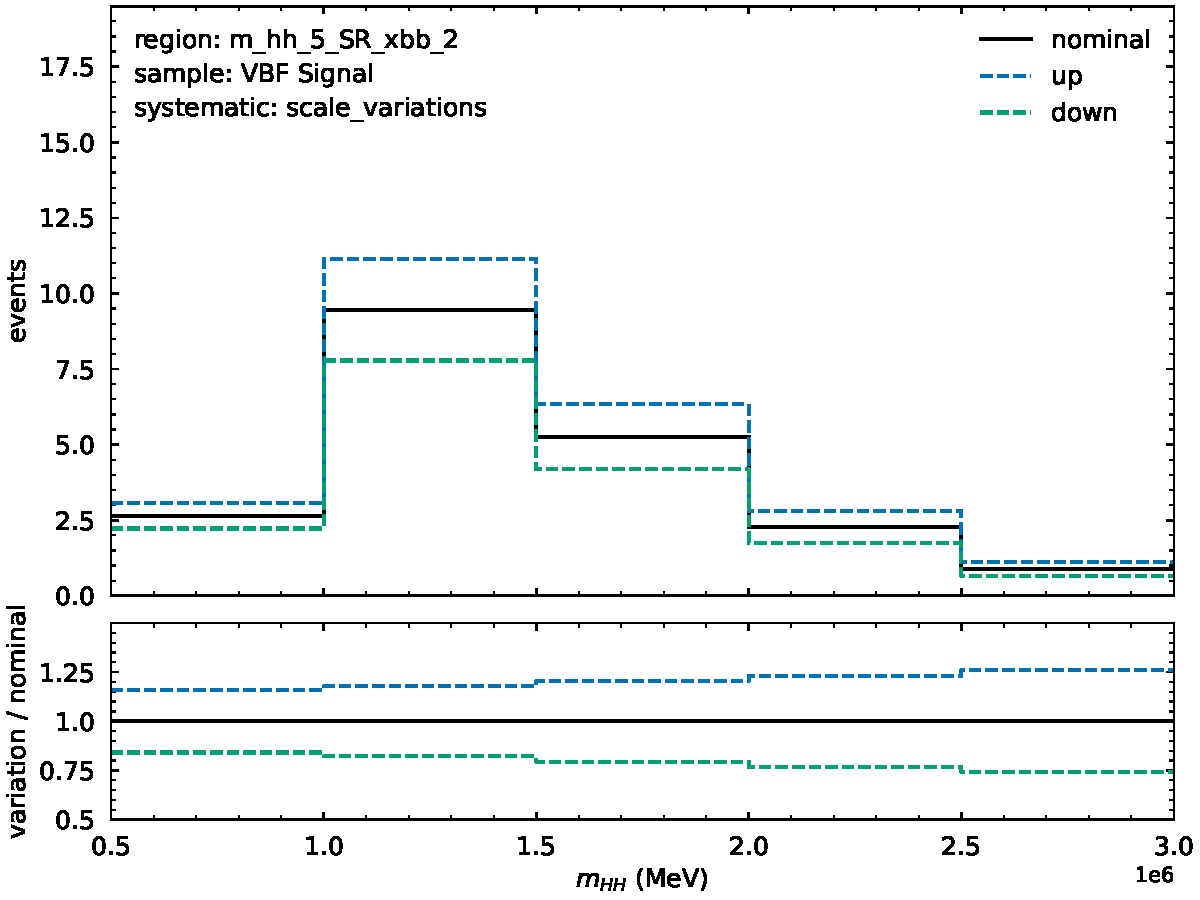
\includegraphics[width=.3\textwidth]{neos_results/m_hh_5_l1cvv0cv1/figures/templates/m_hh_5_SR_xbb_2_VBF-Signal_scale_variations.pdf}}
    \subfigure[]{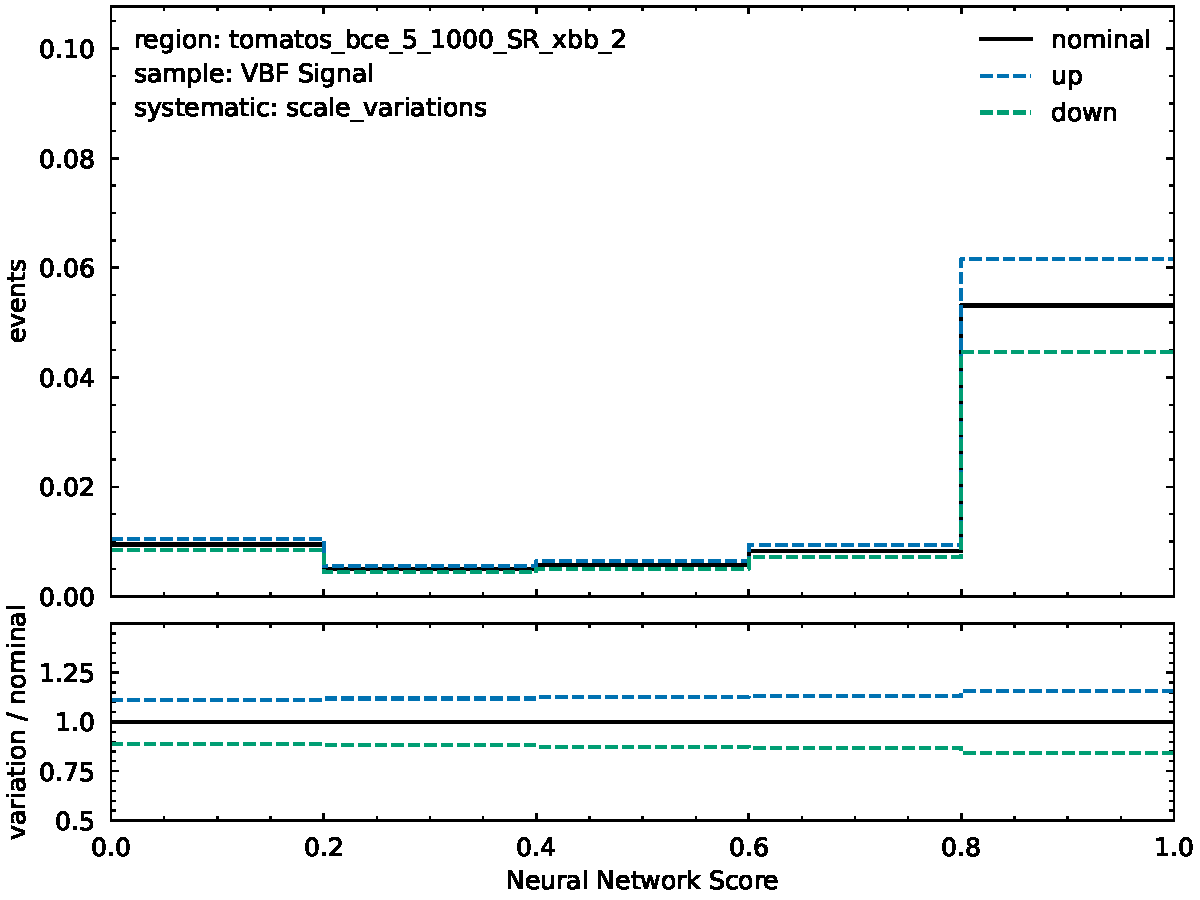
\includegraphics[width=.3\textwidth]{neos_results/tomatos_bce_5_1000_l1cvv0cv1/figures/templates/tomatos_bce_5_1000_SR_xbb_2_VBF-Signal_scale_variations.pdf}}
    \subfigure[]{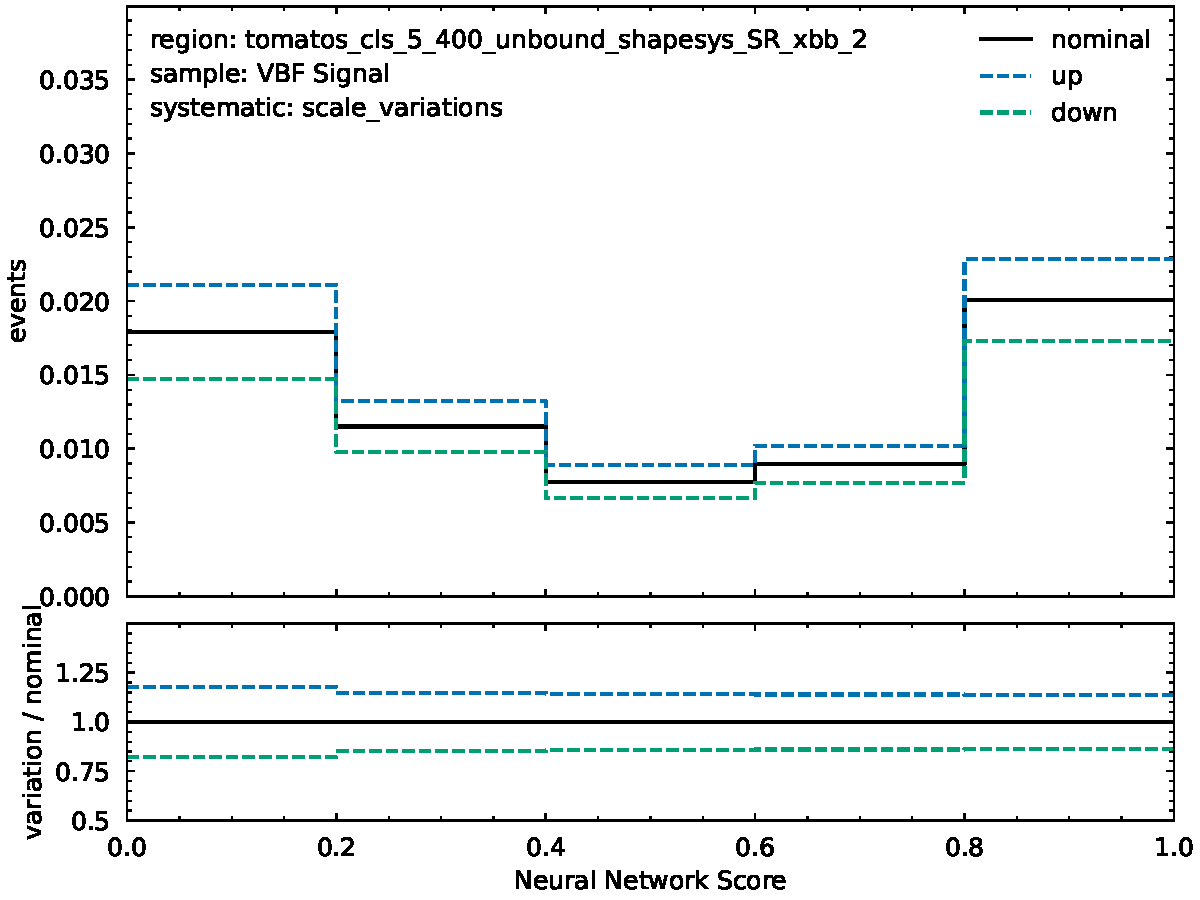
\includegraphics[width=.3\textwidth]{neos_results/tomatos_cls_5_400_unbound_shapesys_l1cvv0cv1/figures/templates/tomatos_cls_5_400_unbound_shapesys_SR_xbb_2_VBF-Signal_scale_variations.pdf}} \\
    \caption[]{Uncertainties (2/2) for columns left to right: $\mhh$, \ac{bce}-trained \ac{nn}, \ac{neos}-trained \ac{nn}. Top to bottom: background shape uncertainty and the envelope of scale variations. Details about their estimation are found in chapter \ref{ch:systematics}. \red{check again if these contain all} }
    \label{fig:neos_validation_uncertaintes_2}
\end{figure}

Histograms and their uncertainties are shown in figure \ref{fig:neos_pre_post_fit} before and after fitting. All models display more constrained postfit uncertainties.
\begin{figure}
    \centering
    \subfigure[]{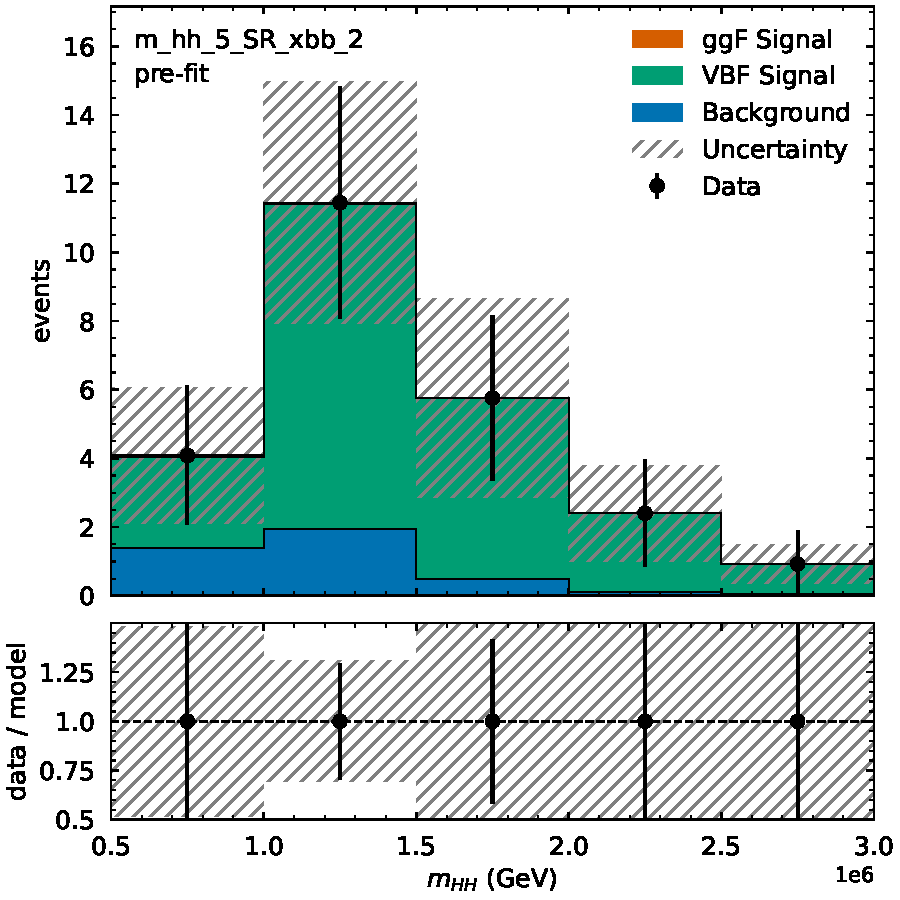
\includegraphics[width=.3\textwidth]{neos_results/m_hh_5_l1cvv0cv1/figures/m_hh_5_SR_xbb_2_prefit.pdf}}
    \subfigure[]{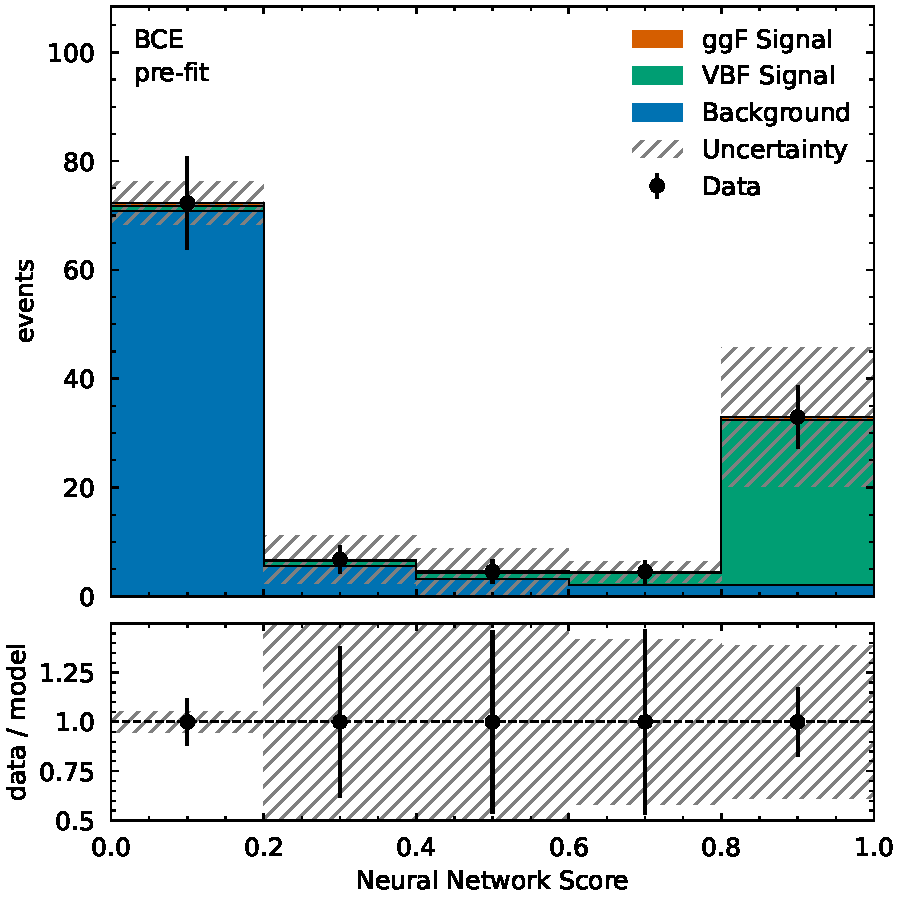
\includegraphics[width=.3\textwidth]{neos_results/tomatos_bce_5_1000_l1cvv0cv1/figures/tomatos_bce_5_1000_SR_xbb_2_prefit.pdf}}
    \subfigure[]{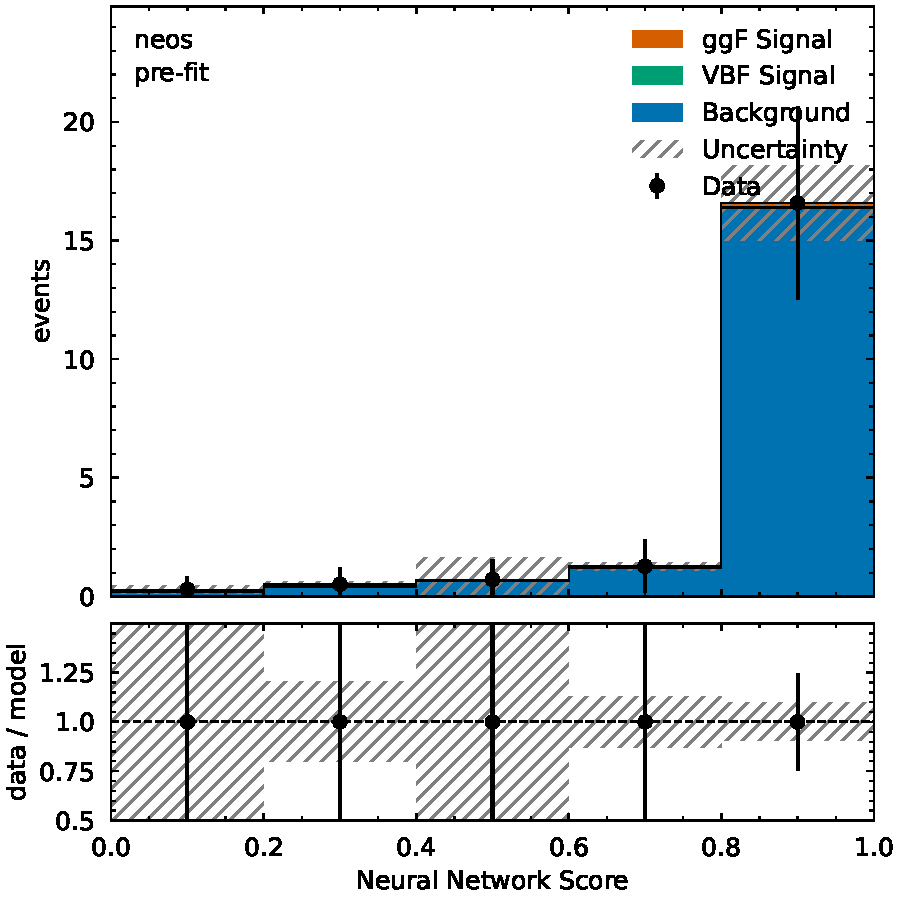
\includegraphics[width=.3\textwidth]{neos_results/tomatos_cls_5_400_unbound_shapesys_l1cvv0cv1/figures/tomatos_cls_5_400_unbound_shapesys_SR_xbb_2_prefit.pdf}} \\
    \subfigure[]{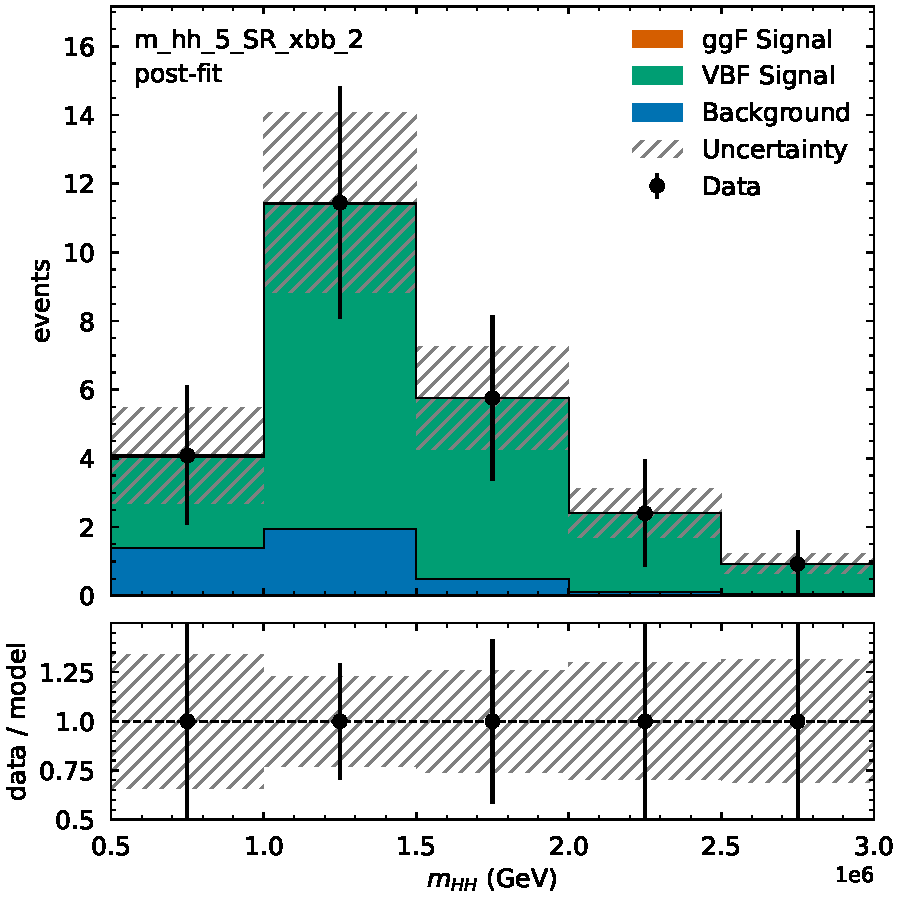
\includegraphics[width=.3\textwidth]{neos_results/m_hh_5_l1cvv0cv1/figures/m_hh_5_SR_xbb_2_postfit.pdf}}
    \subfigure[]{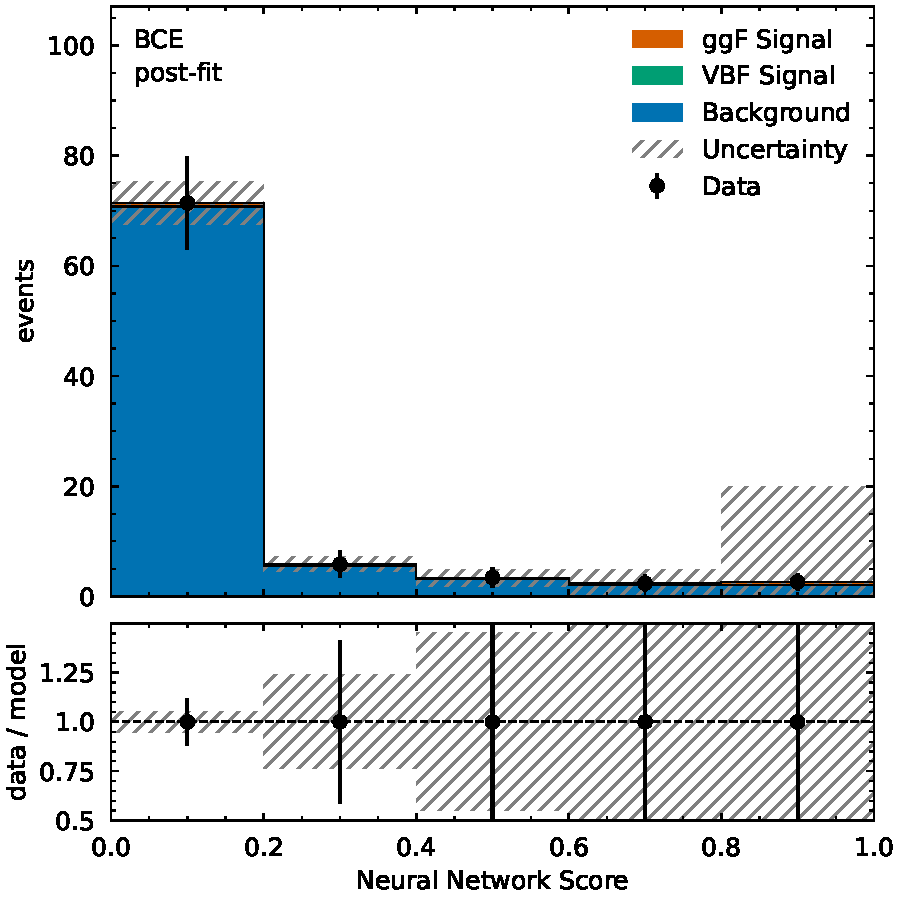
\includegraphics[width=.3\textwidth]{neos_results/tomatos_bce_5_1000_l1cvv0cv1/figures/tomatos_bce_5_1000_SR_xbb_2_postfit.pdf}}
    \subfigure[]{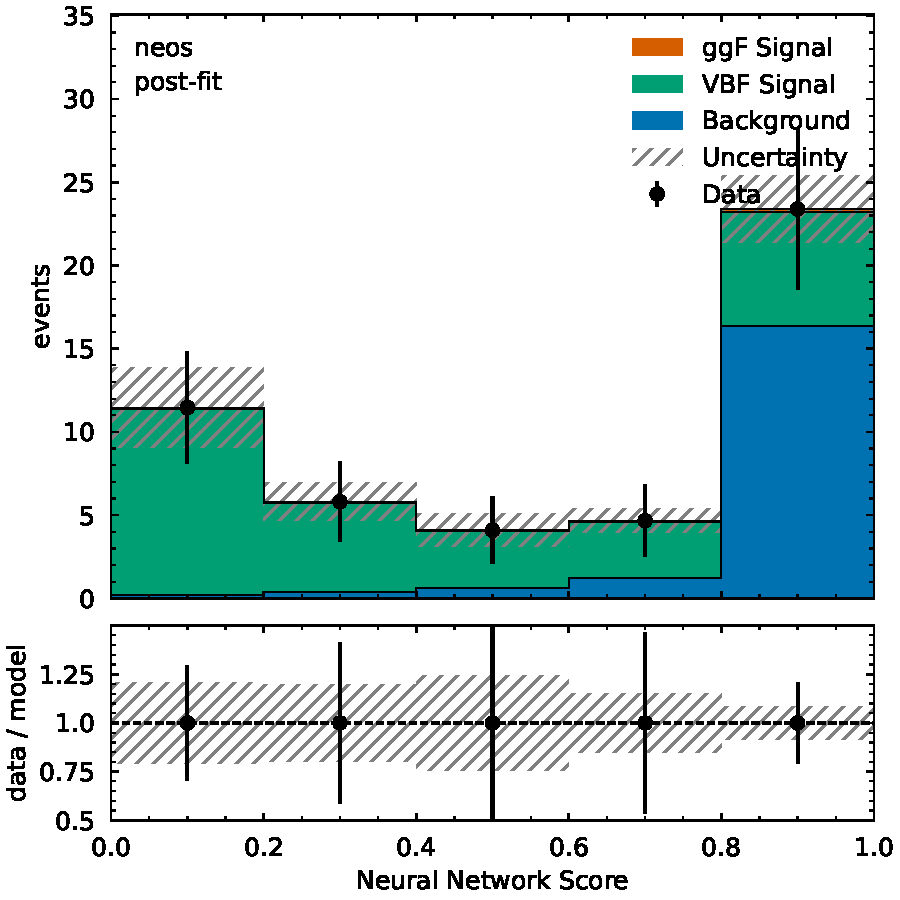
\includegraphics[width=.3\textwidth]{neos_results/tomatos_cls_5_400_unbound_shapesys_l1cvv0cv1/figures/tomatos_cls_5_400_unbound_shapesys_SR_xbb_2_postfit.pdf}}
    \caption[]{Pre- \textbf{(a)-(c)} and Postfit \textbf{(d)-(f)} histogram for columns left to right: $\mhh$, \ac{bce}-trained \ac{nn}, \ac{neos}-trained \ac{nn} }
    \label{fig:neos_pre_post_fit}
\end{figure}

Nuisance parameter rankings for the \ac{bce}-trained and neos-trained \ac{nn} are shown in figure \ref{fig:neos_valid_ranking_bce} and \ref{fig:neos_valid_ranking_cls}. Since \ac{neos} optimizes on the fit, nuisance parameter pre- and postfit impacts are generally smaller compared to the \ac{bce}-trained \ac{nn}. The dominating uncertainties are generally in this analysis the GN2X version of the $X\rightarrow bb$ tagger and the scale variations, detailed in chapter \ref{ch:systematics}. The most prominent feature of \ac{neos} in this analysis is its ability to adjust the \ac{nn} with respect to the background estimate moving it in the ranking even below the dominating uncertainties. In turn the \ac{bce}-trained \ac{nn} shows that the background estimate shape is overestimated as can be seen by a small pull uncertainty and the pre- and postfit impacts on the signal strength.

% \begin{figure}
%     \centering
%     \includegraphics[width=1\textwidth]{neos_results/m_hh_5_l1cvv0cv1/figures/ranking.pdf}
%     \caption[]{}
%     \label{fig:neos_valid_ranking_m_hh}
% \end{figure}
\begin{figure}
    \centering
    \includegraphics[width=1\textwidth]{neos_results/tomatos_bce_5_1000_l1cvv0cv1/figures/ranking.pdf}
    \caption[]{}
    \label{fig:neos_valid_ranking_bce}
\end{figure}
\begin{figure}
    \centering
    \includegraphics[width=1\textwidth]{neos_results/tomatos_cls_5_400_unbound_shapesys_l1cvv0cv1/figures/ranking.pdf}
    \caption[]{}
    \label{fig:neos_valid_ranking_cls}
\end{figure}

Furthermore the correlation matrices for the models in figures \ref{fig:correlation_matrix_m_hh}, \ref{fig:correlation_matrix_bce} and \ref{fig:correlation_matrix_cls} reveal a strong correlation of the signal strength to the uncertainties of the GN2X $(X\rightarrow bb)$ tagger. When error propagating covariances contribute to the overall uncertainty as can be seen by calculating the variance of a function $f(\theta_1, \theta_2)$ depending on two parameters with their individual $\sigma_1,\sigma_2$ uncertainties
\begin{equation}
    \text{Var}(f(\theta_1, \theta_2)) = \left( \frac{\partial f}{\partial \theta_1} \right)^2 \sigma_1^2 + \left( \frac{\partial f}{\partial \theta_2} \right)^2 \sigma_2^2 + 2 \left( \frac{\partial f}{\partial \theta_1} \right) \left( \frac{\partial f}{\partial \theta_2} \right) \sigma_{12}.
\end{equation}
Thus if parameters $\theta_1, \theta_2$ are correlated in some way the cross-term \(2 \left( \frac{\partial f}{\partial \theta_1} \right) \left( \frac{\partial f}{\partial \theta_2} \right) \sigma_{12}\) contributes to the overall uncertainty. \ac{neos} therefore seems to be able to decorrelate uncertainties. \red{ist das zu mutmaßlich, wir sehen das zwar, aber es ist kein beweis.}

\begin{figure}
    \centering
    \includegraphics[width=1\textwidth]{neos_results/m_hh_5_l1cvv0cv1/figures/correlation_matrix.pdf}
    \caption[]{}
    \label{fig:correlation_matrix_m_hh}
\end{figure}
\begin{figure}
    \centering
    \includegraphics[width=1\textwidth]{neos_results/tomatos_bce_5_1000_l1cvv0cv1/figures/correlation_matrix.pdf}
    \caption[]{}
    \label{fig:correlation_matrix_bce}
\end{figure}
\begin{figure}
    \centering
    \includegraphics[width=1\textwidth]{neos_results/tomatos_cls_5_400_unbound_shapesys_l1cvv0cv1/figures/correlation_matrix.pdf}
    \caption[]{}
    \label{fig:correlation_matrix_cls}
\end{figure}

Expected limits on the cross-section for \ktwov=0 and the \ac{sm} \ac{vbf} signal are shown in figure \ref{fig:neos_valid_brazil_limits}. For the \ktwov=0 signal the relative improvement of the \ac{neos} approach compared to \mhh is about \qty[]{35}{\percent} whereas in relation to the \ac{bce}-trained \ac{nn} the improvement linearly ranges between \qty[]{5}{\percent} and \qty[]{20}{\percent} with a nominal expected limit improvement of \qty[]{10}{\percent} as shown in figure \ref{fig:neos_valid_brazil_limits}(c). Decreased performance of \ac{neos} evaluated on the \ac{sm} signal suggests the necessity of a reoptimization for the \ac{sm} signal hypothesis \red{explore? or should we drop k2v=1 here? though question will arise anyway in hh4b i guess}
\begin{figure}
    \centering
    \subfigure[]{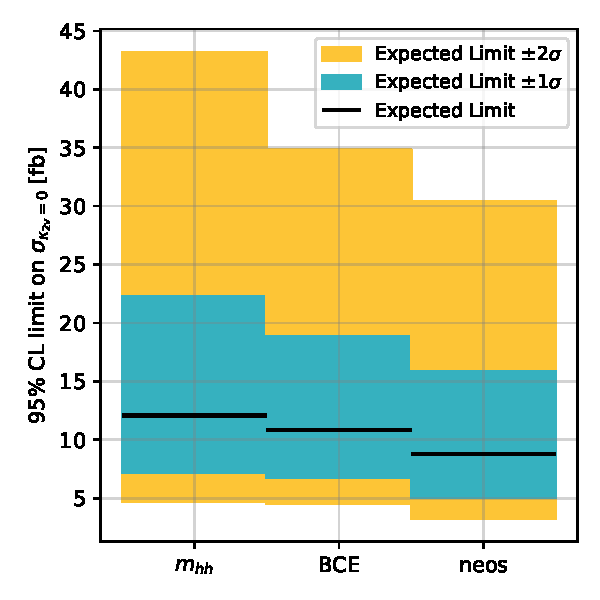
\includegraphics[width=.47\textwidth]{neos_results/brazil_limits_k2v0.pdf}}
    \subfigure[]{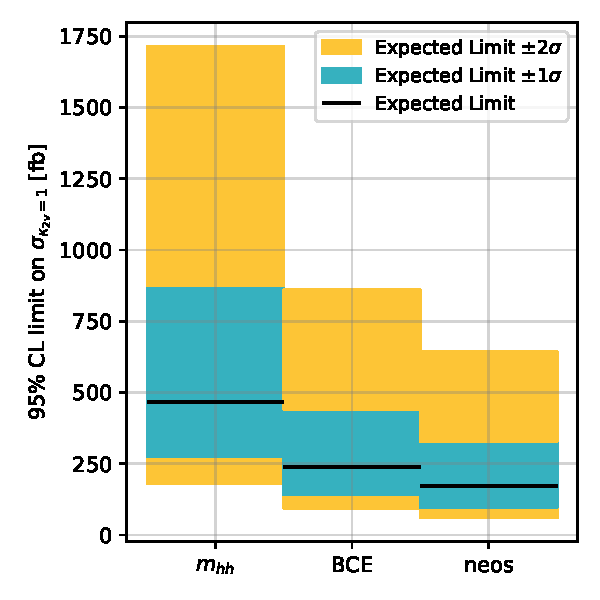
\includegraphics[width=.47\textwidth]{neos_results/brazil_limits_k2v1.pdf}}\\
    \subfigure[]{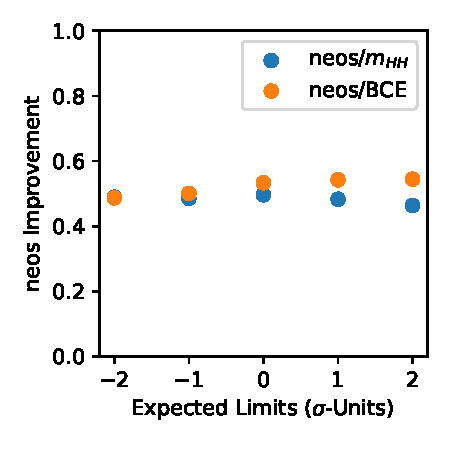
\includegraphics[width=.4\textwidth]{neos_results/relative_limits_k2v0.pdf}}
    \caption[]{Cross-sectional limits on the nominal (a) \ac{vbf} \ktwov=0 and (b) \ac{sm} \ac{vbf} $\ktwov=1$ signal. (c) Relative improvements on expected limits of neos to $m_{HH}$ and the \ac{bce}-trained model for the \ktwov=0 signal hypothesis.}
    \label{fig:neos_valid_brazil_limits}
\end{figure}

With the linear combination of \ac{vbf} signal hypotheses as explained in section \ref{sec:linear_combination} a \ktwov scan for the three models is conducted with results shown in figure \ref{fig:neos_valid_k2v_scan}. The constrained limits for \ktwov are summed up in table \ref{tab:neos_valid_k2v_constraints} with a relative improvement of neos to \ac{bce}-trained \ac{nn} (\mhh) of \qty[]{10}{(27)\percent} on the lower limit and \qty[]{3}{(9)\percent}. 
\red{show overlay here in final part only brazil scan}
\begin{figure}
    \centering
    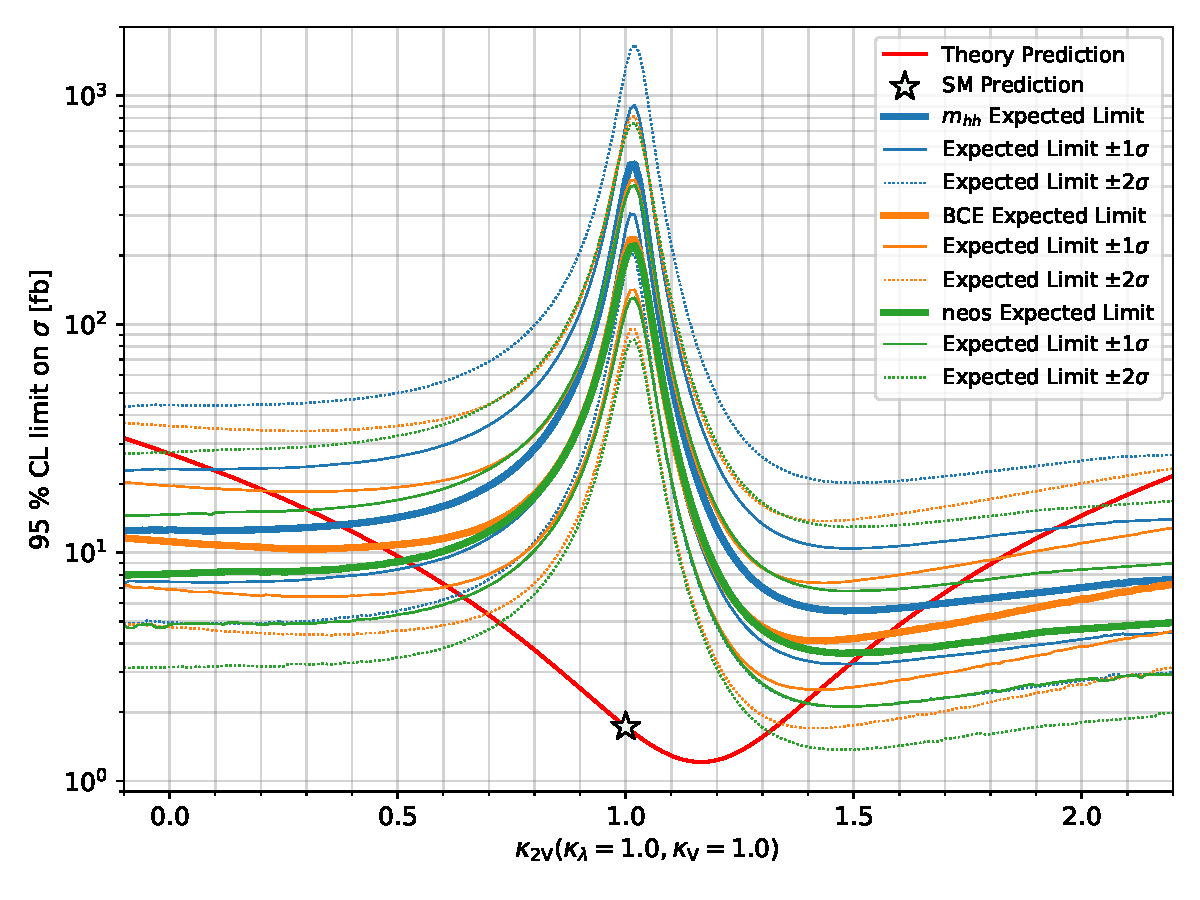
\includegraphics[width=1\textwidth]{neos_results/k2v_scan_limits_overlay_neos_validation.pdf}
    \caption[]{Expected cross-section limits depending on \ktwov for the three models.}
    \label{fig:neos_valid_k2v_scan}
\end{figure}
\begin{table}[htbp]\label{tab:neos_valid_k2v_constraints}
    \centering
    \caption{Expected constraints on \ktwov for the three models.}
    \begin{tabular}{c|c|c}
                                  & Lower \ktwov Limit & Upper \ktwov Limit  \\\hline
        \mhh                      & 0.37               & 1.65                \\
        \ac{bce}-trained \ac{nn}  & 0.46               & 1.57                \\
        \ac{neos}-trained \ac{nn} & 0.51               & 1.52                \\
    \end{tabular}
\end{table}
can see crux of situation, blindly going for Asimov significance, can not account for uncertainties

slight mismatch between nominal sm and linear combined

implementing pdf alphas was not worth the computational overhead of 100 samples, involves a lot of samples with basically no effect

zwei plots brazil limits, k2v0 und sm for the three models
m hh also in addition with old cuts to be fair.
the improvement is blah

neos cut optimization know about unceratinteis/bkg estimate.

limit overlay




auch zeigen sample kombinierungsplot für alle?




better numerical stability if unbound shape sys estiamted unbound


could benefit from a retraining/reoptimization for different \ktwov


warum nicht auf s/b optimieren, kennt zwar keine unsicherheiten, would need histogramming?.


The previous analysis used a more loose cut here, to potentially increase statistics and improve the background estimate. However a test with different cuts displays no improvement against the cuts optimized on the Asimov significance.



gradient verstärken für bkg estiamte oder so